% #55 v2: extended Wilson line terminology + dual-sector hierarchy + Appendix C
% 10.5281/zenodo.19800797 (original v1 record; update on resubmission)

\documentclass[%
 reprint, amsmath,amssymb, aps, prb, ]{revtex4-2}
% Basic packages
\usepackage{graphicx}
\usepackage{bm}
% Quantum-mechanics notation
\usepackage{physics}
% Hyperlinks
\usepackage[colorlinks=true,
            linkcolor=blue, filecolor=blue, urlcolor=blue, citecolor=blue]{hyperref}
% Caption settings
\usepackage{caption}
\captionsetup[figure]{
    justification=raggedright, labelfont={bf}, name={Fig.}, labelsep=period }
\captionsetup[table]{
    labelfont={bf}, name={Table}, labelsep=period }
% Number equations by section
\numberwithin{equation}{section}
% Typography adjustments
\tolerance=1000
\emergencystretch=1em
\hyphenpenalty=3000
\exhyphenpenalty=3000
\flushbottom
% Microtypography
\usepackage[final]{microtype}
\usepackage{ragged2e}  % for \justifying command
% For \midrule, \addlinespace, and \bottomrule
\usepackage{booktabs}
\usepackage{enumitem}
% Theorem environment
\usepackage{amsthm}
\newtheorem{theorem}{Theorem}[section]
% Code listings
\usepackage{listings}
\usepackage{xcolor}
\definecolor{backcolour}{rgb}{0.96,0.97,0.98}
\definecolor{deepblue}{rgb}{0,0,0.5}
\definecolor{deepgreen}{rgb}{0,0.5,0.3}
\definecolor{deepgray}{rgb}{0.4,0.4,0.4}
\definecolor{stringcolor}{rgb}{0.2,0.4,0.6}
\lstdefinestyle{pythonstyle}{
    backgroundcolor=\color{backcolour}, commentstyle=\color{deepgreen}\itshape, keywordstyle=\color{deepblue}\bfseries, numberstyle=\tiny\color{deepgray}, stringstyle=\color{stringcolor}, basicstyle=\ttfamily\footnotesize, breakatwhitespace=false, breaklines=true, captionpos=b, keepspaces=true, numbers=left, numbersep=5pt, showspaces=false, showstringspaces=false, showtabs=false, tabsize=2, language=Python, frame=single, rulecolor=\color{deepgray} }
\lstset{style=pythonstyle}
\usepackage{tikz}
\usetikzlibrary{arrows.meta, calc, 3d, shadings, positioning, decorations.pathmorphing}

% --- Custom Macros ---
\newcommand{\omZB}{\omega_{\text{ZB}}}
\newcommand{\EphS}{E_{\text{ph}}}
\newcommand{\Egrad}{\Delta E_{\text{AB}}}
\newcommand{\FF}{\mathbf{F}}
\newcommand{\WL}{\mathcal{W}}
\newcommand{\hodge}{\star}
\newcommand{\lambdaC}{\lambda_{\mathrm{C}}}
\newcommand{\vZB}{v_{\mathrm{ZB}}}

\begin{document}

\title{Four Functions of the Open Wilson Line in the 0-Sphere Model:\\
Phase-History Carrier, Gauge Localization, Holonomy Composition,\\
and Boundary Data Generating Both Maxwell and Metric Sectors}

\author{Satoshi Hanamura}
\date{April 29, 2026}

\begin{abstract}
The open Wilson line $\WL[A\!\to\!A'] = \int_A^{A'}\Pi$ has emerged as the central structural object of the 0-Sphere model's line-integral ontology. Earlier papers in the series have introduced the notion of line integrals as primary observables, compared open-path and closed-loop transport, identified the internal phase as an internal gauge connection, established the helical thermal geodesic of the photon sphere, and, in the companion paper, derived Maxwell electrodynamics as a low-energy continuum limit in which the open Wilson line is the primary observable, the field-strength 2-form $F = d\Pi$ is a derived curvature, and Maxwell theory itself emerges only at scales $\ell \gg \lambdaC$. The present paper does not add new physical equations to this development; it provides a structural analysis. We identify four logically distinct functions performed by the same object $\WL[A\to A']$: (i) it carries the physical phase history accumulated by the photon sphere along an open helical thermal geodesic; (ii) it localizes the gauge redundancy of the internal 1-form $\Pi$ to the two kernel endpoints $\mathbf{r}_A$ and $\mathbf{r}_{A'}$, converting gauge invariance from a distributed field-theoretic redundancy into a boundary-relative property; (iii) it composes closed-loop observables---the Aharonov--Bohm phase, Berry-type holonomies, magnetic flux---as differences between pairs of open path integrals sharing endpoints; and (iv) it supplies the boundary data from which the continuum description of both sectors of the theory is reconstructed: the smooth 1-form field of classical electromagnetism in the flat-space limit, and the spacetime metric through the Synge reconstruction formula $g_{\mu\nu}(x) = \partial_{A\mu}\partial_{B\nu}\mathcal{S}_s(x_A,x_B)|_{\text{coincidence}}$. The fourth function thus completes the ontological hierarchy established in the companion paper by extending it from a single derived branch (Maxwell) to a bifurcating structure that supports both the electromagnetic and gravitational continuum sectors from the same root. Throughout this analysis the object $\WL[A\to A']$ is understood as a \emph{0-Sphere extended Wilson line}: it inherits the geometric form of the conventional quantum-field-theoretic Wilson line but reorganizes every physical input---integrand, path, endpoints, parametrization---around the components of the 0-Sphere model. The four functions are not independent postulates; they are distinct facets of the single structural choice of treating $\int_A^{A'}\Pi$ as the primary physical observable in place of the field-strength tensor $F_{\mu\nu}$. We examine the consistency of this perspective with the Wu--Yang formulation of gauge theory and with Kothawala's bi-tensor programme in quantum gravity, and we specify the technical requirements of each remaining stage in the broader programme.
\end{abstract}

\maketitle

%-------------------------------------------------------------
\section{Introduction}
\label{sec:intro}
%-------------------------------------------------------------

The 0-Sphere model has progressively reorganized its theoretical apparatus around a single conceptual move: treating line integrals along physical trajectories as the primary observables of the theory~\cite{hanamura29, hanamura31, hanamura40, hanamura41}. The conceptual basis for this reorganization was established in a sequence of three earlier papers, which together articulated the line-integral viewpoint at increasing levels of generality. Reference~\cite{hanamura29} demonstrated, through the explicit case of Thomas precession on the thermal geodesic, that the relevant geometric quantity is the line integral of a \emph{connection} along proper time rather than the curvature of the spatial path or the integration of a fiber bundle itself, with the result that a spinorial $2\pi$ phase accumulates internally even when the external trajectory is straight. Reference~\cite{hanamura30} extended this principle to the gravitational sector by reinterpreting the Bianchi identity as the integrability condition for line integrals of the connection to be globally well-defined, and the Einstein field equation as a posterior consistency condition---a geometric checksum verifying that the accumulated connection-based structure remains self-consistent---rather than as a primary dynamical law. Reference~\cite{hanamura31} consolidated the viewpoint into a unifying principle: the Aharonov--Bohm effect, the Berry phase, and Wilson loops are not separate quantum, geometric, and gauge-theoretic phenomena but instances of the same underlying structure, in which the physically meaningful observable is a line integral of a connection along a path. A complementary line of development, initiated in Ref.~\cite{hanamura22}, established that the Zitterbewegung frequency $\omZB$ is not a formal artefact of the Dirac equation but a physical internal oscillation of the electron governed by proper time $\tau$, and showed that this internal oscillator is therefore subject to gravitational time dilation in the same manner as a classical clock. The same reference derived a specific quantitative prediction: the proper-frame Zitterbewegung frequency at satellite altitude exceeds that at Earth's surface by a fractional amount $\delta\nu/\nu \approx 5.29 \times 10^{-10}$, corresponding to an absolute frequency shift $\Delta\nu \approx 2.64 \times 10^{9}\,\text{Hz}$ in the natural Zitterbewegung scale $\nu_{\text{ZB}} \sim 5 \times 10^{18}\,\text{Hz}$. This prediction, recorded in 2025 with concrete numerical values and a definite experimental geometry (the GPS-orbit-versus-surface comparison employed in atomic-clock relativistic timekeeping~\cite{ashby2003}), establishes that the line-integral ontology of the 0-Sphere framework is not a purely structural reformulation: it carries a falsifiable empirical signature accessible at scales already routinely operational in satellite navigation. Within this reorganization, the open Wilson line
\begin{equation}
\WL[A \to A'] \equiv \int_{\gamma:\,\mathbf{r}_A}^{\mathbf{r}_{A'}} \Pi
\label{eq:WL_intro}
\end{equation}
has acquired a central status. It appears in the geometric phase structure of spinorial transport~\cite{hanamura29}, in the systematic comparison of open-path and closed-loop observables~\cite{hanamura43}, in the analysis of holonomy sufficiency and torsion~\cite{hanamura45}, in the Maxwell derivation developed in the companion paper~\cite{hanamura54}, in the identification of the internal phase with an internal gauge connection~\cite{hanamura17, hanamura45}, and, most recently, in the generalized Synge world function $\mathcal{S}(x_A,x_B) = \int_{\Gamma_{\text{ext}}}\mathcal{A}_\mu\,dx^\mu$ from which Ref.~\cite{hanamura51} proposes the spacetime metric as a coincidence limit of mixed second derivatives.

A terminological clarification is in order before proceeding. The term ``Wilson line'' originates in the quantum field-theoretic literature on gauge theories, where it denotes the path-ordered exponential $\mathcal{P}\exp(ig\int_\gamma A_\mu^a T^a\,dx^\mu)$ acting as an operator on the Hilbert space of charged matter, employed primarily as an analytical tool for confinement, scattering amplitudes, and lattice regularization. The object $\WL[A\to A']$ studied here inherits the geometric form of this construction---the integral of a connection 1-form along a directed path with specified endpoints---but its physical content is reorganized around the components of the 0-Sphere model: the integrand $\Pi$ is the Berry connection 1-form of the internal state bundle rather than a non-Abelian gauge potential on a background spacetime; the path is the unique helical thermal geodesic $\Gamma_{\text{ext}}$ established in Ref.~\cite{hanamura51} rather than an arbitrary mathematical curve; the endpoints $\mathbf{r}_A, \mathbf{r}_{A'}$ are the physically determined kernel positions before and after one inter-kernel energy-exchange cycle rather than free parameters; and the temporal phase $\omZB t$ is internalized within the Hamiltonian identity of the energy partition~\cite{hanamura01} rather than imposed externally as a parametrization of the loop. In this sense, $\WL[A\to A']$ is best understood as a \emph{0-Sphere extended Wilson line}---related to its quantum-field-theoretic counterpart by the form of the integrand but distinguished from it by physical determination of every input. Throughout this paper we use ``Wilson line'' as shorthand for this extended object except where direct comparison with the conventional construction makes the distinction relevant; a detailed comparison is provided in Appendix~\ref{app:terminology}. The companion paper~\cite{hanamura54} has placed this extended Wilson line at the apex of an ontological hierarchy in which the field-strength curvature $F = d\Pi$ is derived and Maxwell electrodynamics emerges as a low-energy continuum limit at scales $\ell \gg \lambdaC$. The present paper extends this hierarchy by showing that the same primary observable supports a second derived branch leading to the spacetime metric, and by identifying the four functional roles through which the extended Wilson line occupies its apex position.

In these earlier developments, particular aspects of the Wilson line are invoked as each physical application requires: its role as carrier of accumulated phase in Ref.~\cite{hanamura29}, its directional asymmetry $A\to B \neq B\to A$ in Ref.~\cite{hanamura43}, its relation to holonomy and torsion in Ref.~\cite{hanamura45}, its connection to Maxwell electrodynamics through $F = d\Pi$ in Ref.~\cite{hanamura54}, and its role as a generalized Synge world function from which the metric is reconstructed in Ref.~\cite{hanamura51}. What has not yet been provided is a systematic account of the Wilson line as a single multi-functional object whose various uses follow from one structural postulate.

The present paper supplies that account. We analyze $\WL[A\to A']$ as performing four logically distinct functions simultaneously, and show that the appearance of these four functions in the same object is not a coincidence but a direct consequence of choosing $\int_A^{A'}\Pi$ as the primary observable in place of the conventional field-strength tensor. The four functions are:
\begin{enumerate}
\item \textit{Phase-history carrier}: the Wilson line records the phase accumulated by the photon sphere along its actual open helical trajectory~\cite{hanamura51};
\item \textit{Gauge localization}: it converts the gauge freedom of $\Pi$, distributed over spacetime in the conventional picture, into a boundary-relative freedom localized at $\mathbf{r}_A$ and $\mathbf{r}_{A'}$;
\item \textit{Holonomy composition}: it constructs closed-loop observables such as the Aharonov--Bohm phase and magnetic flux as differences between two open paths sharing endpoints, rather than as primary objects in their own right;
\item \textit{Boundary data for the continuum sectors}: it provides the source data from which both continuum descriptions are reconstructed---the smooth 1-form field of classical electromagnetism in the flat-space limit~\cite{hanamura54}, and the spacetime metric via the Synge reconstruction formula of Ref.~\cite{hanamura51} in curved space.
\end{enumerate}
These four functions overlap in content but not in logical role. Once we place the decomposition explicitly in view, several consequences follow. First, the Wilson line is identified as an ontological primitive rather than a calculational device: it is not introduced to simplify existing expressions but to replace them. Second, the compatibility of this stance with Wu--Yang gauge theory~\cite{WuYang1975}, with non-Abelian formulations of Yang--Mills~\cite{YangMills1954}, and with the bi-tensor quantum-gravity programme of Kothawala~\cite{Kothawala2023} can be stated precisely. Third, the fourth function exhibits a dual-sector structure: the electromagnetic and gravitational descriptions of the theory are not two separate sectors requiring independent postulates, but two limits of the same boundary-data structure. The flat-space limit of the fourth function generates the Maxwell sector developed in Ref.~\cite{hanamura54}; the curved-space limit generates the metric sector initiated in Ref.~\cite{hanamura51}. The dual-sector hierarchy displayed in Sec.~\ref{sec:boundary} (Eq.~\eqref{eq:hierarchy_55} and Fig.~\ref{fig:hierarchy}) extends the single-branch hierarchy of Ref.~\cite{hanamura54} into the bifurcating structure that the four-function decomposition makes explicit.

This last observation changes the status of the staged programme that leads from the electromagnetic analysis to the gravitational analysis. The Synge world function $\mathcal{S}$ is not a distant future object but an existing component of the 0-Sphere framework, introduced in Ref.~\cite{hanamura51} together with the flat-space consistency check and the connection to the Kothawala bi-tensor programme~\cite{Kothawala2023}. What remains to complete the metric-emergence proof is the explicit evaluation in curved spacetime, together with the Wilson-line action principle and the non-Abelian extension. The staged character of the programme therefore refers not to whether metric emergence is achievable in principle but to the specific technical gaps that remain within a construction already under development.

The paper is organized as follows. Section~\ref{sec:history} analyzes the Wilson line as a carrier of physical phase history, with attention to the helical geometry of the actual 0-Sphere trajectory established in Ref.~\cite{hanamura51}. Section~\ref{sec:gauge} treats the gauge localization function and its connection to the clock-synchronization picture of U(1) gauge theory~\cite{hanamura17, WuYang1975}. Section~\ref{sec:composition} develops the composition of closed-loop observables from open paths, building on the open-path versus closed-loop analysis of Ref.~\cite{hanamura43} and the Aharonov--Bohm construction~\cite{Aharonov1959, Tonomura1986}. Section~\ref{sec:boundary} develops the boundary-data function and its dual-sector structure, with the Maxwell sector emerging in the flat-space limit~\cite{hanamura54} and the metric sector emerging via the Synge world function $\mathcal{S}$ of Ref.~\cite{hanamura51}, and presents the bifurcating hierarchy that extends the chain established in Ref.~\cite{hanamura54}. Section~\ref{sec:integration} integrates the four functions and identifies their common structural origin. Section~\ref{sec:gauge_theory} relates the present framework to established gauge-theoretic constructions and to the Kothawala bi-tensor programme. Section~\ref{sec:metric_stage} specifies the technical status of each remaining stage of the broader programme. Section~\ref{sec:conclusion} concludes. Appendix~\ref{app:technical} collects technical details; Appendix~\ref{app:staged} specifies the technical prerequisites of each subsequent stage of the programme; Appendix~\ref{app:terminology} provides a detailed comparison between the conventional quantum-field-theoretic Wilson line and the 0-Sphere extended Wilson line studied here.

This paper is written as a conceptual bridge between the line-integral ontology of Ref.~\cite{hanamura31}, the Maxwell application of Ref.~\cite{hanamura54}, and the metric-emergence programme of Ref.~\cite{hanamura51}. Graduate students familiar with classical electromagnetism~\cite{Jackson1998} and elementary differential geometry~\cite{Nakahara2003} should be able to follow the argument without working through the full 0-Sphere paper sequence.

%-------------------------------------------------------------
\section{Function 1: Phase-History Carrier}
\label{sec:history}
%-------------------------------------------------------------

The first function of the open Wilson line is to carry the phase history accumulated by the photon sphere along the inter-kernel thermal geodesic. This function is implicit in every appearance of $\WL[A\to A']$ in the 0-Sphere literature; its logical status and its geometric content deserve explicit discussion.

\subsection{The physical mechanism}

The 0-Sphere model describes the electron as a composite structure consisting of two kernel sites, connected by a photon sphere that cycles energy between them at the Zitterbewegung frequency $\omZB$~\cite{hanamura01, hanamura33}. The internal energy partition~\cite{hanamura01}
\begin{align}
E_A &= E_0\cos^4\!\!\left(\tfrac{\omZB t}{2}\right), \label{eq:EA}\\
E_B &= E_0\sin^4\!\!\left(\tfrac{\omZB t}{2}\right), \label{eq:EB}\\
\EphS &= \tfrac{1}{2}E_0\sin^2(\omZB t), \label{eq:Eph}
\end{align}
produces the inter-kernel radiation gradient
\begin{equation}
\Egrad = E_A - E_B = E_0\cos(\omZB t),
\label{eq:grad}
\end{equation}
which drives the photon sphere along a continuous trajectory from one kernel to the other. As the photon sphere traverses this open thermal geodesic, the internal 1-form $\Pi$ integrates along its path, giving the Wilson line
\begin{equation}
\WL(t) = \int_{\mathbf{r}_A}^{\mathbf{r}_{A'}}\Pi = W_0 \sin(\omZB t)
\label{eq:WL_dynamical}
\end{equation}
as the quadrature response of a resonantly driven harmonic phase (see Appendix~\ref{app:technical}).

\subsection{The helical structure of the trajectory}

A decisive refinement of the physical picture is provided in Ref.~\cite{hanamura51}: the thermal geodesic between successive kernel positions is not a planar oscillation but a three-dimensional helix. Two independent velocity scales are present. The transverse Zitterbewegung speed, $\vZB \approx 0.04\,c$, is anchored to the anomalous magnetic moment through $\gamma = 1 + a_e$~\cite{hanamura10, hanamura47} and controls the rotational component of the photon sphere's motion. The longitudinal pitch speed $v_{\text{pitch}} \sim c$, set by the Compton-scale kernel separation $\Delta x \sim \lambdaC$, controls the advance of the helix along the propagation axis. Their ratio $v_{\text{pitch}}/\vZB \approx 25$ is fixed by the two-kernel architecture without free parameters.

The helical geometry has two structural consequences for the Wilson line as a phase-history carrier. First, the integration in Eq.~\eqref{eq:WL_dynamical} is not along a straight line or a planar curve, but along the unique extremal helical arc $\Gamma_{\text{ext}}$ connecting $\mathbf{r}_A$ to $\mathbf{r}_{A'}$. The uniqueness of this arc is secured by a chain of geometric results established in Ref.~\cite{hanamura51}: the non-arcwise-connectivity of $S^0 = \{A,B\}$ is repaired by the photon sphere $S^n$ ($n \geq 1$), the Bonnet--Myers theorem applied to the photon-sphere curvature $K \sim \lambdaC^{-2}$ bounds the diameter by $\pi r \sim \lambdaC$ and thereby establishes the confinement domain $\mathcal{D}$ of Ref.~\cite{hanamura33} as a theorem rather than an assumption, and non-antipodality of the kernels on the resulting compact manifold ensures the uniqueness of the geodesic. Second, the integrand $\Pi$ acquires a concrete physical interpretation: it is the Berry connection 1-form $\mathcal{A}_\mu$ whose holonomy along the helical arc records the spinorial phase generated by Thomas precession~\cite{hanamura26, hanamura29}. The identification $\Pi = \mathcal{A}_\mu\,dx^\mu$ is the geometric content of the phase-history carrier function within the 0-Sphere framework.

\subsection{Proper-time governance and gravitational sensitivity}
\label{sec:propertime}

A further consequence of treating the Wilson line as a phase-history carrier, rather than as a formal phase factor, is that the parameter $t$ in Eq.~\eqref{eq:WL_dynamical} is not a coordinate label but the proper time $\tau$ of the photon sphere along its helical trajectory. Reference~\cite{hanamura22} established this point explicitly: the Zitterbewegung frequency $\omZB$ is the inverse natural timescale of a physical internal oscillator confined within the photon-sphere domain, and the dynamical relation $\WL(\tau) = W_0 \sin(\omZB \tau)$ is therefore governed by the proper-time interval accumulated along the worldline of the kernel--photon-sphere--kernel cycle, in direct parallel with the proper-time governance of any classical clock subject to the standard relativistic identity
\begin{equation}
\frac{d\tau}{dt} = \sqrt{1 - \frac{2GM}{rc^2}}
\label{eq:proper_time}
\end{equation}
in a Schwarzschild geometry of mass $M$. The same identity that yields the gravitational redshift of atomic transition frequencies in laboratory and satellite atomic clocks~\cite{ashby2003, ludlow2015} therefore applies, mutatis mutandis, to the internal Zitterbewegung oscillator: when observed from a distant coordinate frame, the apparent frequency of the internal oscillation depends on the gravitational potential at which the electron is located.

This identification has two structural consequences for the present analysis. First, the Wilson line of Eq.~\eqref{eq:WL_dynamical} is not a parametric oscillation in some abstract auxiliary time but a proper-time-governed physical history, with the implication that the same geometric object that records gauge phase along the trajectory simultaneously records the gravitational time-dilation experienced along it. Function 1 (phase-history carrier) is therefore not merely a record of internal phase: it is a record of internal phase indexed by proper time, and as such inherits the gravitational sensitivity of any proper-time-governed process. Second, the Wilson line acquires a concrete experimental signature: the comparison of $\WL$-derived observables between regions of different gravitational potential should yield a definite, calculable difference set by the standard general-relativistic factor of Eq.~\eqref{eq:proper_time}. The quantitative form of this signature, together with its place within the dual-sector hierarchy developed in Sec.~\ref{sec:boundary}, is taken up in detail in Sec.~\ref{sec:experimental_signature}; here we record only that the proper-time governance of $\omZB$ established in Ref.~\cite{hanamura22} is the structural ingredient through which the metric sector of Function 4 acquires its first concrete experimental test.

\subsection{Why the path is necessarily open}

A further structural point, established in Ref.~\cite{hanamura43} and already implicit in the Lorentz-contraction analysis of Ref.~\cite{hanamura47}, is that the endpoint $\mathbf{r}_{A'}$ at which the photon sphere arrives after one energy-exchange cycle is spatially distinct from the starting point $\mathbf{r}_A$:
\begin{equation}
\mathbf{r}_{A'} \neq \mathbf{r}_A.
\label{eq:open}
\end{equation}
The kernel never returns exactly to its point of departure, because the electron as a whole is always in motion relative to any external observer. The thermal geodesic $\gamma: \mathbf{r}_A \to \mathbf{r}_{A'}$ is therefore not a closed loop but an open helical arc.

This openness is not a contingent feature of the specific dynamical setting. Even when the center-of-mass trajectory of the electron is externally constrained to oscillate or remain bounded, the internal thermal geodesic between successive kernel positions remains open. The kernel reference point after recondensation carries a non-retracing phase history relative to the one before departure. What is categorically open, in the 0-Sphere framework, is the internal phase structure rather than the center-of-mass trajectory.

This geometric fact underlies the function of the Wilson line as a phase-history carrier. If the path were closed, the accumulated phase would collapse to a holonomy, losing the distinction between the phase history and its endpoint value. Because the path is open, $\WL[A\to A']$ contains more information than any closed-loop quantity: it specifies which open trajectory was traversed, not merely what phase was accumulated around some closed circuit.

\subsection{The history-content of $\WL$}

To make the history content precise, consider two open helical arcs $\gamma_1$ and $\gamma_2$ connecting the same endpoints $\mathbf{r}_A$ and $\mathbf{r}_{A'}$ but traversed under different conditions. Their Wilson lines differ by
\begin{equation}
\WL[\gamma_1] - \WL[\gamma_2] = \int_{\gamma_1} \Pi - \int_{\gamma_2} \Pi.
\label{eq:history_diff}
\end{equation}
This difference is gauge-invariant and, by Stokes' theorem, equal to the flux of $F = d\Pi$ through the surface bounded by the closed curve $\gamma_1 \cup \overline{\gamma_2}$. The Wilson line therefore encodes not only the endpoint phase but the cumulative effect of the field $F$ on the specific path taken. This is what we mean by ``phase history'': the Wilson line records the photon sphere's passage through the field, not merely the initial and final states.

The distinction between phase-history and endpoint-phase has practical consequences throughout the remaining functions. In Ref.~\cite{hanamura54}, the electric field is obtained as the temporal derivative of $\WL(t)$, which is defined only if the history is smoothly parametrized. The magnetic field is obtained as the transverse variation of $\WL$ over a family of parallel helical arcs, which again requires the full history rather than merely an endpoint value. In Ref.~\cite{hanamura51}, the metric tensor is obtained from mixed second derivatives of the symmetrized Wilson-line integral with respect to its endpoint positions---again requiring the full history encoded in the open arc. Both sectors of the continuum theory, electromagnetic and gravitational, ultimately rely on the history content supplied by Function 1.

\subsection{Comparison with the closed-loop holonomy picture}

In the conventional treatment of gauge theory, the physically relevant object associated with a gauge field is the holonomy around a closed loop~\cite{WuYang1975, Nakahara2003}. The open-path observable $\WL[A\to A']$ has no independent status; it is gauge-dependent unless closed. The 0-Sphere framework reverses this priority. The open Wilson line, whose gauge dependence is localized at the endpoints (Sec.~\ref{sec:gauge}), is taken as primary; closed-loop holonomies are derived by comparison (Sec.~\ref{sec:composition}).

The justification for this reversal is not abstract. The physical process represented by the Wilson line---the photon sphere traversing the inter-kernel helical arc during one radiation--recondensation cycle---has a definite physical endpoint at $\mathbf{r}_{A'} \neq \mathbf{r}_A$. There is no physical process corresponding to the photon sphere returning to its exact starting point. The closed loop, viewed in this framework, is a mathematical device for extracting gauge-invariant information, not a physical trajectory. The open path is the physical trajectory.

%-------------------------------------------------------------
\section{Function 2: Gauge Localization at the Endpoints}
\label{sec:gauge}
%-------------------------------------------------------------

The second function of the open Wilson line is to localize the gauge redundancy of the internal 1-form $\Pi$ to the two kernel endpoints, in a form that renders gauge invariance a boundary-relative property rather than a distributed redundancy over spacetime.

\subsection{Gauge transformations of the Wilson line}

Under a smooth redefinition of the phase reference, $\Pi \to \Pi + d\chi$, the path integral $\WL[A\to A']$ transforms as
\begin{equation}
\WL[A\to A'] \;\to\; \WL[A\to A'] + \chi(\mathbf{r}_{A'}) - \chi(\mathbf{r}_A).
\label{eq:WL_gauge}
\end{equation}
The transformation is structurally different from the pointwise gauge transformation of the vector potential $A_\mu \to A_\mu + \partial_\mu \chi$ in conventional electromagnetism. In the latter, the gauge function $\chi$ enters at every point of spacetime, and the redundancy is a property of the field configuration everywhere. In Eq.~\eqref{eq:WL_gauge}, only the values of $\chi$ at the two kernel positions appear. The entire distributed gauge freedom of $\Pi$ has collapsed to a two-point boundary data structure.

Under the identification $\Pi = \mathcal{A}_\mu\,dx^\mu$ with the Berry connection developed in Ref.~\cite{hanamura51}, Eq.~\eqref{eq:WL_gauge} expresses the fact that the generalized Synge functional $\mathcal{S}(x_A, x_B)$ is defined up to a boundary correction determined by the phase conventions at the two kernel events. This is the form in which gauge freedom enters the metric-emergence construction of Ref.~\cite{hanamura51}: the symmetrized combination $\mathcal{S}_s$ used in the reconstruction formula $g_{\mu\nu} = \partial_{A\mu}\partial_{B\nu}\mathcal{S}_s|_{\text{coincidence}}$ is insensitive to any boundary correction that is antisymmetric in the endpoint labels, and the symmetric part of any boundary correction reduces to a constant overall shift that drops out of the mixed second derivative.

\subsection{Connection to clock synchronization}

The structure of Eq.~\eqref{eq:WL_gauge} admits a direct physical interpretation. The values $\chi(\mathbf{r}_A)$ and $\chi(\mathbf{r}_{A'})$ represent independent choices of phase reference at the two kernel positions, with the difference $\chi(\mathbf{r}_{A'}) - \chi(\mathbf{r}_A)$ reflecting the relative phase convention between them. This is the clock-synchronization picture of U(1) gauge symmetry developed in Ref.~\cite{hanamura17}: gauge transformations are resynchronizations of internal clocks at different spatial positions.

Within the 0-Sphere framework, the clock-synchronization picture acquires a physical basis. The kernels are themselves internal clocks of the electron, ticking at the Zitterbewegung frequency $\omZB$~\cite{hanamura22, hanamura33}. A gauge transformation corresponds to adjusting the zero-phase convention at each kernel independently. The Wilson line $\WL[A\to A']$ measures the phase accumulated during transport from the $A$ clock to the $A'$ clock, expressed relative to the chosen conventions. The freedom to change conventions appears entirely at the endpoints, because that is where the two clocks are located.

\subsection{The physical origin of gauge freedom}

This gauge-localization function has a further consequence: it identifies the origin of U(1) gauge freedom with the topology of the source structure. The source of the electromagnetic sector in the 0-Sphere model is a zero-sphere $S^0$, consisting of the two isolated kernel points. Gauge transformations act on the phase reference at each point of $S^0$ independently. The gauge group U(1) emerges as the structure group of phase references compatible with the two-point source topology.

This view is structurally related to the perspective of Wu and Yang~\cite{WuYang1975}, who recognized that the gauge-invariant content of an electromagnetic field configuration is carried by phase factors $\exp(ie\int A\cdot dx/\hbar)$ along paths, rather than by the local value of $A_\mu$ itself. The 0-Sphere framework makes a stronger claim: the phase factor is carried not along an arbitrary mathematical path but along the specific physical helical trajectory of the photon sphere, and the gauge freedom is not an abstract redundancy but a physical freedom in how one chooses phase conventions at the endpoints of this trajectory.

\subsection{Invariance as a property of pairs of paths}

A physically measurable quantity must be invariant under all gauge transformations of the form Eq.~\eqref{eq:WL_gauge}. For a single Wilson line $\WL[\gamma]$, this requires the boundary term to vanish, which it does only if $\chi$ is constrained to equal a fixed value at $\mathbf{r}_A$ and $\mathbf{r}_{A'}$. In a general gauge theory, no such global constraint exists, and $\WL[\gamma]$ alone is not gauge-invariant.

The resolution is that physically measurable quantities are not single Wilson lines but \emph{differences} between Wilson lines sharing endpoints:
\begin{equation}
\Delta\WL[\gamma_1, \gamma_2] \equiv \WL[\gamma_1] - \WL[\gamma_2].
\label{eq:delta_WL}
\end{equation}
Because both $\WL[\gamma_1]$ and $\WL[\gamma_2]$ transform with the same boundary term under Eq.~\eqref{eq:WL_gauge}, the difference is gauge-invariant. This invariance is a natural consequence of the gauge-localization structure: the boundary data at $\mathbf{r}_A$ and $\mathbf{r}_{A'}$ cancels in any comparison of paths that share those endpoints.

The requirement that physical observables be constructed from pairs of open paths leads directly to the third function of the Wilson line.

%-------------------------------------------------------------
\section{Function 3: Holonomy Composition}
\label{sec:composition}
%-------------------------------------------------------------

The third function of the open Wilson line is to serve as the constituent from which closed-loop observables are composed. The closed loop, which in conventional gauge theory plays the role of the primary gauge-invariant object~\cite{WuYang1975, Nakahara2003}, is derived in the present framework as a combination of two open paths.

\subsection{Closed loops as composites}

Consider two open paths $\gamma_1$ and $\gamma_2$ sharing endpoints $\mathbf{r}_A$ and $\mathbf{r}_{A'}$. Reversing the orientation of $\gamma_2$ and appending it to $\gamma_1$ produces a closed curve:
\begin{equation}
C_{12} = \gamma_1 \cup \overline{\gamma_2}.
\label{eq:C12}
\end{equation}
The integral of $\Pi$ around $C_{12}$ is then
\begin{equation}
\oint_{C_{12}} \Pi = \int_{\gamma_1} \Pi - \int_{\gamma_2} \Pi = \Delta\WL[\gamma_1, \gamma_2].
\label{eq:loop_as_diff}
\end{equation}
The closed-loop integral is thus exhibited as the difference of two open-path Wilson lines. It is not postulated as an independent object; it is constructed by comparison.

This is the inverse of the usual logical order. In the conventional treatment, one begins with a closed loop and interprets it as enclosing flux via Stokes' theorem. Here one begins with two physical open trajectories and recognizes that their comparison produces a closed-loop quantity. The open paths are the physical primitives; the closed loop is a bookkeeping device for extracting their gauge-invariant content.

\subsection{The Aharonov--Bohm phase}

The Aharonov--Bohm effect~\cite{Aharonov1959} provides a concrete physical instance of this composition. Two electrons travel along distinct paths $\gamma_1$ and $\gamma_2$ from a source at $\mathbf{r}_A$ to a detector at $\mathbf{r}_{A'}$, in a region where the magnetic field $\mathbf{B}$ is everywhere zero but the vector potential $\mathbf{A}$ is not. The measured interference shift is
\begin{equation}
\Delta\phi_{\text{AB}} = \frac{e}{\hbar}\left(\int_{\gamma_1} \Pi - \int_{\gamma_2} \Pi\right) = \frac{e}{\hbar}\,\Delta\WL[\gamma_1, \gamma_2].
\label{eq:AB_diff}
\end{equation}
By Stokes' theorem this equals $(e/\hbar)\Phi_B$, where $\Phi_B$ is the magnetic flux through the surface bounded by $C_{12}$. The effect was confirmed experimentally by Tonomura \emph{et al.}~\cite{Tonomura1986}.

In the conventional interpretation, Eq.~\eqref{eq:AB_diff} is seen as evidence that the gauge-invariant holonomy $\oint \Pi$ is the primary observable. In the 0-Sphere interpretation, the same equation is seen as evidence that the open path integrals $\WL[\gamma_1]$ and $\WL[\gamma_2]$ are the primary observables, and the holonomy arises as their difference.

\subsection{Berry phase and the spinorial sector}

The Berry phase~\cite{Berry1984} arises when a quantum system is transported adiabatically around a closed loop in parameter space. Within the 0-Sphere model, Berry-phase physics occupies a distinct sector from the electromagnetic Wilson-line physics: it governs the spinorial degree of freedom of the kernel, which accumulates phase around genuinely closed trajectories with $\mathbf{r}_{\text{end}} = \mathbf{r}_{\text{start}}$~\cite{hanamura26, hanamura29}. The 4$\pi$ periodicity characteristic of spinorial transport reflects the SU(2) double cover of SO(3)~\cite{hanamura45}.

The relation between the electromagnetic (Wilson) sector and the spinorial (Berry) sector was analyzed in Ref.~\cite{hanamura43}, which provided the first systematic comparison of open-path and closed-loop observables within the 0-Sphere framework. The conclusion established there is that the two sectors use structurally different path topologies and produce structurally different physical outputs, and must not be conflated. The function of the Wilson line as holonomy composer, as described in this section, applies specifically to the electromagnetic sector where the paths are open. The spinorial sector requires a separate but analogous analysis in which the primary objects are closed-loop holonomies of the SU(2) connection~\cite{hanamura45}.

\subsection{Magnetic flux as a derived concept}

By a natural extension of the composition argument, the magnetic flux $\Phi_B$ through a surface is not an independent primitive but a derived quantity:
\begin{equation}
\Phi_B = \int_{S_{12}} F = \int_{S_{12}} d\Pi = \oint_{C_{12}} \Pi = \Delta\WL[\gamma_1, \gamma_2].
\label{eq:flux_derived}
\end{equation}
Each equality represents a step in the derivation from the primary open-path observables. The magnetic flux is obtained by Stokes' theorem from the closed-loop integral, which is obtained by composition from the two open Wilson lines. The gauge-invariant flux through a region of space is thus ultimately a difference between phase histories carried by two physical trajectories.

This chain of derivations realizes, in the specific context of the 0-Sphere electromagnetic sector, the unifying principle of Ref.~\cite{hanamura31}: that the Aharonov--Bohm effect, the Berry phase, and Wilson loops, which conventional physics classifies as separate quantum, geometric, and gauge-theoretic phenomena, are in fact instances of the same underlying structure in which the physically meaningful observable is a line integral of a connection. Reference~\cite{hanamura31} stated this principle at the level of comparative analysis across canonical examples; the present analysis develops it into operational form by assigning specific logical roles to specific line-integral constructions---with the open path as primitive and the closed loop as composite---and by exhibiting magnetic flux, holonomy, and the Aharonov--Bohm phase as derived quantities within a single chain of compositions originating in the open Wilson line. Function 3 is thus the operational realization, within the 0-Sphere electromagnetic sector, of the unifying line-integral principle established in Ref.~\cite{hanamura31}.

%-------------------------------------------------------------
\section{Function 4: Boundary Data Generating the Continuum Sectors}
\label{sec:boundary}
%-------------------------------------------------------------

The fourth function of the open Wilson line is to supply the boundary data from which the continuum descriptions of the theory are reconstructed. Two such continuum descriptions are relevant within the 0-Sphere framework: the smooth 1-form field $\Pi(\mathbf{r},t)$ of classical electromagnetism, recovered in the flat-space limit $\ell \gg \lambdaC$~\cite{hanamura54}, and the spacetime metric $g_{\mu\nu}(x)$, recovered in curved space through the Synge reconstruction formula of Ref.~\cite{hanamura51}. These two descriptions are the \emph{Maxwell sector} and the \emph{metric sector} of the 0-Sphere framework, respectively. They share a common structural origin: the same Wilson-line data propagated in two different directions generates the two sectors.

\subsection{The scale-separation limit}

The 0-Sphere source has the topology of a zero-sphere $S^0$ consisting of two isolated kernel points separated by the Compton-wavelength scale $2a \sim \lambdaC = \hbar/(m_e c) \approx 2.4 \times 10^{-12}$~m. Following Ref.~\cite{hanamura51}, the photon sphere that bridges these kernel points is modeled as a compact Riemannian manifold with curvature scale set by the Compton wavelength: $K \sim \lambdaC^{-2}$. The Bonnet--Myers theorem then gives a diameter bound $\mathrm{diam} \leq \pi r \sim \lambdaC$, establishing the confinement domain $\mathcal{D}$ of Ref.~\cite{hanamura33} as a geometric consequence rather than an external assumption.

When the observation scale $\ell$ satisfies
\begin{equation}
\ell \gg \lambdaC,
\label{eq:scale_sep}
\end{equation}
the two-point source structure is unresolved, and a smooth continuous description becomes possible. This scale separation is not a lattice limit of the kind employed in lattice gauge theory~\cite{Wilson1974}, in which spacetime itself is discretized. The spacetime of the 0-Sphere model is continuous at all scales; only the source has two-point structure.

\subsection{The Maxwell sector: flat-space limit}

In the flat-space limit, the single Wilson line $\WL(t) = W_0 \sin(\omZB t)$ associated with one inter-kernel trajectory is extended to a smooth 1-form field $\Pi(\mathbf{r},t)$ defined over the observation region. The extension is determined by three conditions: the boundary value $\WL(t)$ supplied at the source, the requirement of macroscopic causality (no superluminal propagation), and the requirement of smoothness at scales $\ell \gg \lambdaC$. Together these conditions select the retarded interpolation
\begin{equation}
\Pi(r,t) = \frac{W_0}{r} \sin\!\left[\omZB\!\left(t - \frac{r}{c}\right)\right],
\label{eq:retarded}
\end{equation}
valid in the far-field region $r > 0$. This expression satisfies the homogeneous wave equation $\Box \Pi = 0$ away from the source and reproduces $\WL(t)$ in the near-field limit $r \to 0$ within the scale-separation resolution. Reference~\cite{hanamura54} develops this sector in full and derives the Maxwell equations as either mathematical identities ($dF = d^2\Pi = 0$) or stationarity conditions of the action $S = -(1/4\mu_0)\int F \wedge \hodge F$.

The structural point is that $\WL(t)$ plays the role of a \emph{boundary condition} rather than a field equation. The field $\Pi(\mathbf{r},t)$ is determined in the bulk by the wave equation, subject to the source-side data supplied by $\WL(t)$. The wave equation itself is not postulated but emerges as a consistency condition on this reconstruction.

\subsection{The metric sector: curved-space recovery via Synge reconstruction}

A second continuum description is recovered from the same boundary data when the flat-space assumption is dropped. A line-integral interpretation of gravitational quantities had already been proposed in Ref.~\cite{hanamura37}, which reinterpreted gravitational potential energy as an internal line-integral quantity $\Theta = \int_\gamma \omega$ accumulated along the worldline, with the connection 1-form $\omega$ identified as an effective U(1) projection of the underlying SU(2) spinorial structure. Reference~\cite{hanamura37} thereby established the physical interpretation that the formal construction of the metric sector here completes: the gravitational sector is governed by line integrals of an internal connection along physical trajectories, with $mgh$-type quantities representing differences in accumulated internal phase rather than energies stored at spatial positions. The open Wilson line, regarded as a function of its endpoint pair, is the generalized Synge world function of Ref.~\cite{hanamura51}:
\begin{equation}
\mathcal{S}(x_A, x_B) \equiv \int_{\Gamma_{\text{ext}}(x_A, x_B)} \mathcal{A}_\mu\, dx^\mu,
\label{eq:synge_def}
\end{equation}
where $\mathcal{A}_\mu$ is the Berry connection 1-form of the 0-Sphere internal state bundle---the formalization of the connection $\omega$ proposed in Ref.~\cite{hanamura37}---and $\Gamma_{\text{ext}}$ is the unique extremal helical arc connecting $x_A$ to $x_B$ whose existence is secured by the Bonnet--Myers result. The functional $\mathcal{S}$ is a real-valued two-point function that vanishes at coincidence ($\mathcal{S}(x,x) = 0$), is antisymmetric under endpoint exchange ($\mathcal{S}(x_B,x_A) = -\mathcal{S}(x_A,x_B)$), and reduces to a proper-time integral in the flat-space limit. Its symmetrization
\begin{equation}
\mathcal{S}_s(x_A, x_B) \equiv \tfrac{1}{2}\!\left[\mathcal{S}(x_A,x_B) + \mathcal{S}(x_B,x_A)\right]
\label{eq:symmetrization}
\end{equation}
retains the metric-generating part of the functional; the antisymmetric part encodes spin and chirality~\cite{hanamura50}. Reference~\cite{hanamura51} then proposes the spacetime metric as the coincidence limit of mixed second derivatives,
\begin{equation}
g_{\mu\nu}(x) \;=\; \partial_{A\mu}\,\partial_{B\nu}\,\mathcal{S}_s(x_A,x_B)\Big|_{x_A = x_B = x},
\label{eq:metric_proposal}
\end{equation}
in direct analogy with the Synge reconstruction theorem for the conventional world function $\sigma(x,x') = \tfrac{1}{2}d^2(x,x')$~\cite{Synge1960, DeWittBrehme1960}. The correspondence is
\begin{align}
\underbrace{\sigma(x_A, x_B)}_{\text{conventional Synge}}
&\;\longleftrightarrow\;
\underbrace{2\,\mathcal{S}(x_A, x_B)}_{\text{0-Sphere phase history}},
\label{eq:synge_correspondence}
\end{align}
with the squared geodesic distance of the conventional construction replaced by twice the accumulated phase history of the helical arc.

The flat-space consistency check in Ref.~\cite{hanamura51} verifies that Eq.~\eqref{eq:metric_proposal} reproduces the Minkowski metric $\eta_{\mu\nu}$ in the absence of curvature, using the proportionality $\mathcal{S} \approx \omZB \int_A^B d\tau$ valid when $\mathcal{A}_\mu$ is constant. The explicit evaluation in curved spacetime, which would promote Eq.~\eqref{eq:metric_proposal} from a consistent proposal to a verified reconstruction, is an open task recorded in Ref.~\cite{hanamura51}.

\subsection{Two sectors from one boundary-data function}

The two reconstructions described in the preceding subsections originate in the same boundary data: the open Wilson line $\WL[A\to A']$ supplied at the physical endpoints of the 0-Sphere trajectory. They differ in the direction in which the boundary data is propagated into the continuum, and each yields one of the two continuum sectors of the theory.

The Maxwell sector uses a single Wilson line $\WL(t)$ attached to a single inter-kernel cycle, and propagates it outward in space through a retarded Green-function interpolation. The resulting continuum object is a 1-form field $\Pi(\mathbf{r},t)$ defined over the spacetime region around the source. Differentiating $\Pi$ once with respect to spacetime coordinates yields the field-strength tensor $F = d\Pi$; the equations of motion for $F$ follow as consistency conditions.

The metric sector uses the Wilson line as a function $\mathcal{S}(x_A, x_B)$ of its two endpoints considered as variable spacetime events, and propagates it through variation of the endpoint positions. The resulting continuum object is a two-point function on spacetime. Differentiating $\mathcal{S}_s$ twice with respect to the two endpoints and taking the coincidence limit yields the metric $g_{\mu\nu}$; the Christoffel symbols and curvature tensor follow through the conventional differential chain $g \to \Gamma \to R$.

The structural parallel is exact. In both sectors, the Wilson line is the primary object, an interpolation procedure generates a continuum field or function, and the field equations of the respective sector follow as consistency conditions. What distinguishes the two sectors is only the direction in which the boundary data is propagated: along spacetime in the Maxwell sector, along endpoint pairs in the metric sector. Table~\ref{tab:sectors} summarizes the correspondence.

\begin{table*}[t!]
\centering
\caption{\textbf{Two sectors generated by the boundary-data function: Maxwell and metric reconstructions}}
\label{tab:sectors}
\renewcommand{\arraystretch}{1.4}
\begin{tabular}{p{3.6cm}p{5.5cm}p{5.9cm}}
\toprule
\textbf{Aspect} & \textbf{Maxwell sector} & \textbf{Metric sector} \\
\midrule
Wilson-line role
& Single-trajectory boundary data $\WL(t)$
& Endpoint-pair functional $\mathcal{S}(x_A, x_B)$ \\
\addlinespace[0.3cm]
Propagation direction
& Outward in spacetime (retarded Green function)
& Variation of endpoint positions \\
\addlinespace[0.3cm]
Continuum object
& 1-form field $\Pi(\mathbf{r},t)$
& Two-point function on spacetime \\
\addlinespace[0.3cm]
Derivative structure
& $F = d\Pi$ (once differentiated)
& $g_{\mu\nu} = \partial_{A\mu}\partial_{B\nu}\mathcal{S}_s$ (twice differentiated, coincidence limit) \\
\addlinespace[0.3cm]
Consistency condition
& Maxwell equations
& Einstein equations (emergent) \\
\addlinespace[0.3cm]
Validity regime
& Flat-space limit, $\ell \gg \lambdaC$
& Curved space, $\mathcal{A}_\mu$ position-dependent \\
\addlinespace[0.3cm]
Current status
& Derivation complete~\cite{hanamura54}
& Flat-space check complete~\cite{hanamura51}; curved-space proof open \\
\addlinespace[0.2cm]
\bottomrule
\end{tabular}
\vspace{0.2cm}
\begin{minipage}{0.95\textwidth}
\justifying\footnotesize
The two continuum sectors of the 0-Sphere framework are generated by the same boundary-data function (Function 4 of the Wilson line). They differ only in the direction in which the Wilson-line data is propagated into the continuum: along spacetime coordinates in the Maxwell sector, along endpoint pairs in the metric sector. The Maxwell sector is developed in Ref.~\cite{hanamura54}. The metric sector is initiated in Ref.~\cite{hanamura51}, which establishes the flat-space consistency check; the curved-space proof remains open.
\end{minipage}
\end{table*}

The dual-sector structure admits a direct physical interpretation in terms of the two independent ways in which the kernel configuration can be varied. A variation of the kernel positions $\mathbf{r}_A$ and $\mathbf{r}_{A'}$, with the trajectory between them preserved in structural type, alters the endpoints of the Wilson line and is captured by the metric sector: the change in $\mathcal{S}(x_A, x_B)$ under endpoint variation encodes the change in spacetime geometry between the two events. A variation of the trajectory connecting the two kernels, with the endpoints held fixed, alters the path of the Wilson line and is captured by the Maxwell sector: the change in $\WL[\gamma]$ under path variation encodes the gauge-field content recorded along the traversal. Endpoint variation generates the metric sector; path variation generates the Maxwell sector. The two sectors are two physically distinct ways of perturbing the same Lagrangian data.

\subsection{The dual-sector hierarchy: extension of the line-integral ontology}
\label{sec:hierarchy_extension}

The structural correspondence summarized in Table~\ref{tab:sectors} can be expressed compactly as a hierarchical relation that extends the ontological hierarchy established in Ref.~\cite{hanamura54}. There the Maxwell sector was placed within the chain $\WL = \int_A^{A'}\Pi \to F = d\Pi \to (\mathbf{E},\mathbf{B},\text{Maxwell})$, identifying the open Wilson line as the primary observable, the field-strength 2-form as a derived curvature, and Maxwell electrodynamics as the low-energy continuum limit. The present paper completes this picture by showing that the same primary observable bifurcates into two derived structures, corresponding to the two propagation directions discussed in the preceding subsections:
\begin{align}
&\underbrace{\WL[A\to A'] = \int_A^{A'}\Pi}_{\text{primary observable (Lagrangian data)}}
\notag\\[0.2em]
&\quad\swarrow\qquad\qquad\qquad\searrow\notag\\[0.2em]
&\underbrace{F = d\Pi}_{\text{derived 2-form}}
\qquad\quad
\underbrace{\mathcal{S}(x_A,x_B)}_{\text{two-point functional}}
\notag\\[0.2em]
&\quad\downarrow\qquad\qquad\qquad\quad\downarrow\notag\\[0.2em]
&\underbrace{\text{Maxwell theory}}_{\ell\gg\lambdaC,\;\text{Ref.~\cite{hanamura54}}}
\qquad
\underbrace{g_{\mu\nu} = \partial_{A}\partial_{B}\mathcal{S}_s|_{\text{coinc}}}_{\text{Ref.~\cite{hanamura51}}}.
\label{eq:hierarchy_55}
\end{align}

The left branch reproduces the chain established in Ref.~\cite{hanamura54}: the open Wilson line generates the field-strength 2-form by exterior differentiation, and Maxwell theory emerges in the flat-space limit at scales $\ell \gg \lambdaC$. The right branch was initiated in Ref.~\cite{hanamura51}: the open Wilson line, regarded as a function of its endpoint pair, generates the symmetric two-point functional $\mathcal{S}_s$, whose mixed second derivative at coincidence yields the spacetime metric. Both branches share the same root---the open Wilson line as primary observable---and the structural parallel between them is the content of Function 4 in its dual-sector form. The hierarchy of Eq.~\eqref{eq:hierarchy_55} is therefore not an addition to the ontological structure of the line-integral ontology but its completion: the leftmost level identified in Ref.~\cite{hanamura54} is shown to support both continuum sectors of the theory simultaneously. Figure~\ref{fig:hierarchy} displays the bifurcation visually.

\begin{figure*}[t!]
\centering
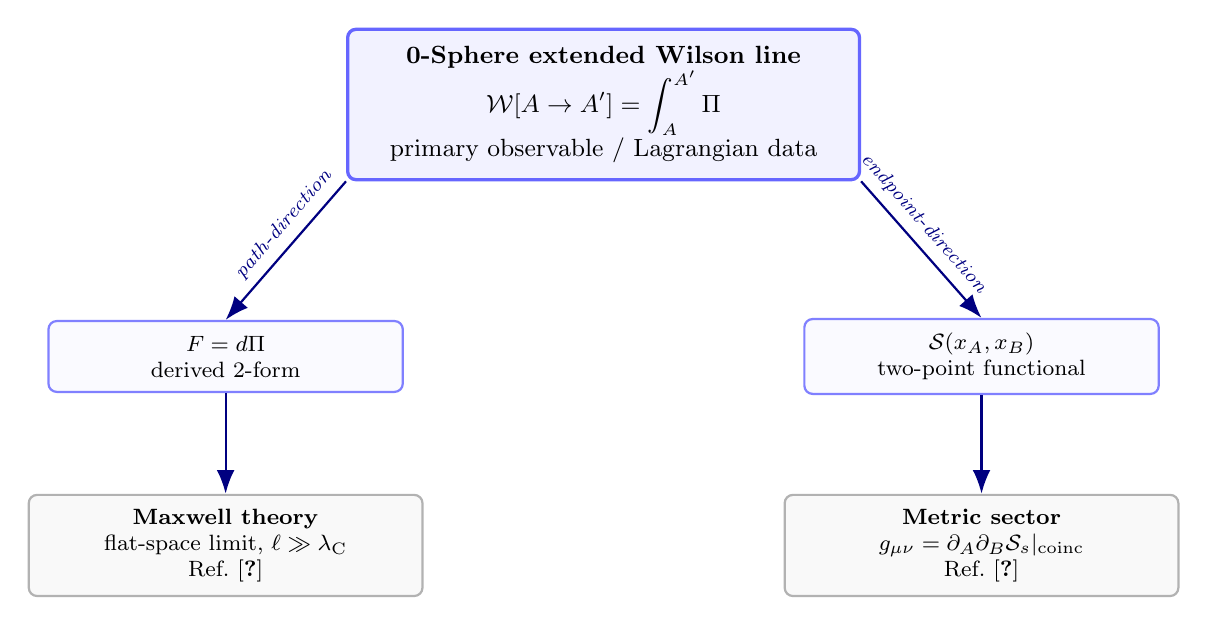
\begin{tikzpicture}[
    node distance=1.2cm,
    rootbox/.style={
        draw=blue!60, fill=blue!5, very thick, rounded corners=3pt,
        align=center, font=\small, inner sep=6pt,
        minimum width=6.5cm, minimum height=1.2cm
    },
    midbox/.style={
        draw=blue!50, fill=blue!2, thick, rounded corners=3pt,
        align=center, font=\footnotesize, inner sep=5pt,
        minimum width=4.5cm, minimum height=0.9cm
    },
    leafbox/.style={
        draw=gray!60, fill=gray!5, thick, rounded corners=3pt,
        align=center, font=\footnotesize, inner sep=5pt,
        minimum width=5.0cm, minimum height=1.0cm
    },
    arrow/.style={-{Latex[length=3mm]}, thick, blue!50!black},
    branchlabel/.style={font=\scriptsize\itshape, text=blue!50!black, midway, sloped, above}
]

% Root node
\node[rootbox] (W) at (0, 0) {%
    \textbf{0-Sphere extended Wilson line}\\
    $\WL[A\to A'] = \displaystyle\int_A^{A'}\Pi$\\
    primary observable / Lagrangian data
};

% Mid-level: F=dPi (left) and S(x_A,x_B) (right)
\node[midbox] (F) at (-4.8, -3.2) {%
    $F = d\Pi$\\
    derived 2-form
};
\node[midbox] (S) at (4.8, -3.2) {%
    $\mathcal{S}(x_A, x_B)$\\
    two-point functional
};

% Bifurcation arrows from root to mid-level
\draw[arrow] (W.south west) -- (F.north) node[branchlabel, pos=0.4] {path-direction};
\draw[arrow] (W.south east) -- (S.north) node[branchlabel, pos=0.4] {endpoint-direction};

% Leaf level: Maxwell (left) and Metric (right)
\node[leafbox] (Max) at (-4.8, -5.6) {%
    \textbf{Maxwell theory}\\
    flat-space limit, $\ell \gg \lambdaC$\\
    Ref.~\cite{hanamura54}
};
\node[leafbox] (Met) at (4.8, -5.6) {%
    \textbf{Metric sector}\\
    $g_{\mu\nu} = \partial_{A}\partial_{B}\mathcal{S}_s|_{\text{coinc}}$\\
    Ref.~\cite{hanamura51}
};

% Vertical arrows down to leaves
\draw[arrow] (F) -- (Max);
\draw[arrow] (S) -- (Met);

\end{tikzpicture}
\caption{The dual-sector hierarchy generated by the open Wilson line. The 0-Sphere extended Wilson line $\WL[A\to A']$ sits at the apex as the primary observable. Path-direction propagation (left branch) generates the field-strength 2-form $F = d\Pi$ and yields Maxwell theory in the flat-space limit~\cite{hanamura54}. Endpoint-direction propagation (right branch) generates the two-point functional $\mathcal{S}(x_A,x_B)$ and yields the spacetime metric through the Synge reconstruction~\cite{hanamura51}. The two branches share the same root and are distinguished only by the direction in which the boundary data is propagated into the continuum. The hierarchy extends the single-branch chain established in Ref.~\cite{hanamura54} to the bifurcating structure that the four-function decomposition makes explicit.}
\label{fig:hierarchy}
\end{figure*}

\subsection{What the boundary-data function accomplishes}

The boundary-data function completes the passage from microscopic to macroscopic description. The other three functions all operate at the microscopic level of individual 0-Sphere trajectories: the phase-history carrier records the trajectory's phase evolution, the gauge localization expresses the freedom at its two endpoints, and the holonomy composition extracts gauge-invariant differences between trajectory pairs. The boundary-data function takes the collection of such microscopic observables and interpolates them into two distinct continuum descriptions, each associated with a different direction of propagation of the boundary data.

Without this fourth function, the Wilson-line description would be formally complete but would not connect to any continuum theory. With it, both classical electromagnetism (the Maxwell sector) and general relativity (the metric sector) emerge as coarse-grained effective descriptions of the microscopic Wilson-line dynamics. The Wilson line is thus both the microscopic physical observable and the common generator of both macroscopic sectors.

\subsection{Experimental signature: gravitational shift of the internal Zitterbewegung clock}
\label{sec:experimental_signature}

The dual-sector structure of Function 4 admits a concrete experimental test that has been recorded with specific numerical values in Ref.~\cite{hanamura22}. The test was formulated several years before the four-function decomposition of the present paper was articulated, and consequently exists in the literature as an independent, dated prediction whose verification or falsification would directly bear on the metric sector of Function 4. The structural significance of this test, and the precision with which the prediction is recorded, are sufficient to warrant a dedicated subsection within the development of Function 4, even though the present paper does not introduce new physical equations. The role of this subsection is twofold: to translate the prediction of Ref.~\cite{hanamura22} into the language of the four-function decomposition, and to make explicit why the existence of this prediction is not an isolated curiosity but a structural consequence of the metric sector being a derived branch of the same Lagrangian primitive that generates the Maxwell sector.

\subsubsection{The prediction in its original formulation}

Reference~\cite{hanamura22} treats the Zitterbewegung frequency $\omZB$ as the natural timescale of a physical internal oscillator confined within the photon-sphere domain of the electron, with the oscillator governed by the proper time $\tau$ of the kernel--photon-sphere--kernel cycle (Sec.~\ref{sec:propertime}). Because $\omZB$ is, in this formulation, a proper-time frequency rather than a coordinate-time frequency, it inherits the standard general-relativistic transformation
\begin{equation}
\frac{d\tau}{dt} = \sqrt{1 - \frac{2GM}{rc^2}}
\label{eq:proper_time_revisit}
\end{equation}
between proper time and coordinate time in a Schwarzschild geometry. When the Zitterbewegung oscillation is observed from a distant coordinate frame, its apparent frequency is shifted by exactly the factor of Eq.~\eqref{eq:proper_time_revisit}, in direct parallel with the gravitational redshift of any other proper-time-governed clock~\cite{ashby2003, ludlow2015}. Reference~\cite{hanamura22} computes the resulting frequency shift between the Earth's surface ($r = R_E = 6.371 \times 10^{6}\,\text{m}$) and a satellite altitude representative of the GPS constellation ($h = 2.02 \times 10^{7}\,\text{m}$, $r_{\text{sat}} = 2.6571 \times 10^{7}\,\text{m}$):
\begin{align}
\left(\frac{d\tau}{dt}\right)_{\!\!\text{Earth}} &\approx 1 - 6.96 \times 10^{-10}, \\
\left(\frac{d\tau}{dt}\right)_{\!\!\text{sat}} &\approx 1 - 1.67 \times 10^{-10}.
\end{align}
The fractional frequency difference between satellite and surface, when both are referred to a common distant coordinate frame, is therefore
\begin{equation}
\frac{\Delta\nu_{\text{ZB}}}{\nu_{\text{ZB}}} \approx 5.29 \times 10^{-10},
\label{eq:fractional_shift}
\end{equation}
which, for the natural Zitterbewegung scale $\nu_{\text{ZB}} \approx 5.0 \times 10^{18}\,\text{Hz}$ associated with the special-relativistic internal velocity $\vZB \approx 0.04\,c$ established in Refs.~\cite{hanamura10, hanamura47, hanamura28}~through the anomalous-magnetic-moment relation $\gamma = 1 + a_e$ and the rotational Lorentz contraction of the photon sphere, corresponds to an absolute coordinate-frame frequency shift
\begin{equation}
\Delta\nu_{\text{ZB}} \approx 2.64 \times 10^{9}\,\text{Hz}
\label{eq:absolute_shift}
\end{equation}
between the surface-bound and orbit-bound electron populations. Equations~\eqref{eq:fractional_shift} and~\eqref{eq:absolute_shift} are the operational form of the prediction. We note that the fractional shift $\delta\nu/\nu$ of Eq.~\eqref{eq:fractional_shift} depends only on the gravitational potential difference between the two locations through Eq.~\eqref{eq:proper_time_revisit} and is independent of the absolute value of $\vZB$; the value of $\vZB$ enters only as a multiplicative factor setting the absolute frequency scale of the predicted shift. Consequently, the prediction is operationally robust under refinements to the absolute determination of $\vZB$: subsequent corrections within the 0-Sphere programme established that the special-relativistic value $v_{e,\text{SR}} = 0.040472\,c$ is governed by Lorentz kinematics alone, with general-relativistic corrections to the internal velocity proving negligible at all physically relevant scales~\cite{hanamura28}; the gravitational shift $\delta\nu/\nu \approx 5.29 \times 10^{-10}$ obtained from Eq.~\eqref{eq:proper_time_revisit} is unaffected by this clarification, since it expresses the gravitational redshift of a proper-time-governed oscillator rather than a general-relativistic correction to the oscillator's intrinsic velocity.

\subsubsection{Translation into the language of the four-function decomposition}

Within the framework of the present paper, the prediction of Ref.~\cite{hanamura22} acquires a structural interpretation that was not articulated in the original formulation. The relation $\WL(\tau) = W_0 \sin(\omZB \tau)$ identified in Function 1 is governed by proper time, and the Wilson-line data $\WL(\tau)$ supplied at the source of the metric sector of Function 4 is therefore a proper-time-governed function. When this data is propagated into the continuum through the endpoint-direction mechanism of Function 4---that is, when the dependence of $\WL$ on the kernel positions $\mathbf{r}_A$ and $\mathbf{r}_{A'}$ as variable spacetime events is taken seriously and used to construct the symmetrized two-point functional $\mathcal{S}_s(x_A, x_B)$ from which the metric is reconstructed via Eq.~\eqref{eq:metric_proposal}---the proper-time character of $\WL$ is inherited by $\mathcal{S}_s$. The resulting two-point functional is sensitive to the gravitational potential at its endpoints precisely because the proper time accumulated along the helical arc connecting them is.

The prediction of Ref.~\cite{hanamura22} can therefore be re-read as the statement that the Wilson-line data sitting at the apex of the dual-sector hierarchy of Eq.~\eqref{eq:hierarchy_55} is itself gravitationally sensitive, and that the metric sector of Function 4 (the right branch of the hierarchy) accordingly inherits this sensitivity in a form that is testable at scales where the underlying internal oscillation is operationally accessible. The Maxwell sector (the left branch) does not exhibit a comparable gravitational signature at leading order, because the field-strength curvature $F = d\Pi$ is constructed by exterior differentiation of $\Pi$ at fixed spacetime points and therefore does not carry the proper-time governance of $\WL$ in a directly observable form; the gravitational sensitivity of the line-integral ontology is concentrated, by the structural logic of the four-function decomposition, in the metric sector. This concentration is one of the structural reasons why the bifurcating hierarchy of Eq.~\eqref{eq:hierarchy_55} has explanatory content beyond mere taxonomic convenience: it predicts which sector should exhibit which class of empirical signature.

\subsubsection{Operational form of the test}

The operational form of the prediction is unusually accessible by the standards of physics that probes the intersection of quantum mechanics and general relativity. The standard general-relativistic factor of Eq.~\eqref{eq:proper_time_revisit} is already routinely implemented in the relativistic timekeeping algorithms of GPS and equivalent global navigation satellite systems, where it produces the well-known fractional shift of order $10^{-10}$ between satellite-borne and ground-based atomic clocks~\cite{ashby2003}. The prediction of Ref.~\cite{hanamura22} is that the same factor applies to the internal Zitterbewegung oscillator of the electron, and that the resulting frequency shift $\Delta\nu_{\text{ZB}} \approx 2.64 \times 10^{9}\,\text{Hz}$ between surface and orbit should be detectable in any experimental scheme capable of resolving the Zitterbewegung scale at the level of $\delta\nu/\nu \sim 10^{-10}$. The technical challenge of such a measurement lies not in the relative precision required---which is comparable to that already achieved in optical-clock comparisons~\cite{ludlow2015}---but in the absolute frequency scale, which lies at $\sim 10^{18}\,\text{Hz}$ in the natural $\omZB \sim m_e c^2/\hbar$ regime and therefore exceeds the direct reach of current frequency-comb spectroscopy. Indirect schemes are conceivable: the sub-cycle anticorrelation signature identified in Ref.~\cite{hanamura54} between the photon-sphere occupation and the electromotive-force quadrature within each $\omZB$ cycle is, in principle, accessible to attosecond spectroscopy; the gravitational modulation of $\omZB$ predicted by Ref.~\cite{hanamura22} would correspondingly modulate the timing of the sub-cycle signature by a fractional amount $\delta t/t \sim 5 \times 10^{-10}$, which sets the precision target for any experimental discrimination between surface-bound and orbit-bound electron ensembles. The combination of the structural prediction of Ref.~\cite{hanamura54} (sub-cycle signature at $\Delta t \sim \pi/\omZB \approx 6.3 \times 10^{-19}\,\text{s}$) with the gravitational modulation of Ref.~\cite{hanamura22} (fractional shift $\sim 5 \times 10^{-10}$) defines a two-dimensional experimental discriminant: a single observation that resolves both the absolute timescale of the internal oscillation and its dependence on gravitational potential would simultaneously test the two branches of the dual-sector hierarchy.

\subsubsection{Structural placement of the prediction}

The prediction of Ref.~\cite{hanamura22} occupies an unusual position within the development of the 0-Sphere line-integral programme. It was formulated in 2025, on the basis of the proper-time governance of $\omZB$ argued for in Refs.~\cite{hanamura01, hanamura11} and the relativistic kinematics of internal motion developed in Refs.~\cite{hanamura10, hanamura47}, well before the four-function decomposition of the present paper or the metric-sector formalism of Ref.~\cite{hanamura51} were articulated in their current form. The structural content of the prediction---that an internal proper-time-governed oscillator is subject to gravitational time dilation in the same manner as a classical clock, and that the resulting fractional frequency shift between two gravitational potentials is given by Eq.~\eqref{eq:fractional_shift}---is independent of any specific determination of the absolute internal velocity $\vZB$, since the gravitational time-dilation factor of Eq.~\eqref{eq:proper_time_revisit} multiplies any proper-time frequency uniformly. It is appropriate to record here that an intermediate stage of the 0-Sphere programme considered the possibility of additional general-relativistic corrections to the absolute value of $\vZB$ itself; this avenue was subsequently re-examined in Ref.~\cite{hanamura28}, which established through dimensional analysis that such corrections are negligible at all physically relevant scales and that $\vZB$ is governed by special-relativistic kinematics alone. The clarification of Ref.~\cite{hanamura28} concerns the determination of the absolute internal velocity, not the gravitational redshift of the proper-time-governed oscillation, and consequently does not affect the structural prediction of a gravitationally-induced fractional shift recorded in Ref.~\cite{hanamura22}, which remains the operative experimental signature of the metric sector. From the standpoint of 2026, the prediction is therefore not an inference drawn from the structural framework of the present paper; it is an antecedent prediction whose physical content the present framework retrospectively organizes. This temporal ordering carries methodological weight: it ensures that any future experimental confirmation of the predicted shift cannot be accommodated by structural adjustments of the four-function decomposition, because the decomposition was not in place when the prediction was made. The prediction, in this sense, constitutes a falsifiable test of the line-integral ontology that is structurally independent of, and prior to, the framework that the present paper develops.

The historical pattern this temporal arrangement instantiates is familiar in physics. Theoretical predictions issued before the structural framework that retrospectively organizes them have, on previous occasions, played decisive roles in the consolidation of new physical theories: the Einstein 1915 prediction of light deflection by the Sun, confirmed by the Eddington 1919 eclipse observation, preceded the full synthesis of general relativity in the form it would later acquire; the Higgs 1964 prediction of a massive scalar boson, confirmed by the ATLAS and CMS observations of 2012, preceded the consolidation of the Standard Model in the form it would later acquire. In neither case was the prediction's verification a direct consequence of the framework in which the verification was eventually interpreted; in both cases, the prediction's verification provided the experimental ground on which the framework was subsequently judged. The position of Ref.~\cite{hanamura22} within the present programme is structurally similar: a quantitative prediction issued in advance of the consolidating framework, whose eventual verification or falsification will bear directly on the empirical standing of that framework. We do not press the analogy with Einstein--Eddington and Higgs--ATLAS/CMS in any quantitative sense, but the structural pattern---prediction first, framework second, verification third---is one of the recognizable patterns by which physics has historically arrived at confidence in its theories.

The placement of the prediction of Ref.~\cite{hanamura22} within Function 4 of the present decomposition therefore serves a definite purpose. It records that the metric sector of the dual-sector hierarchy is not merely a structural proposal awaiting completion in Stage 3 of the staged programme (Sec.~\ref{sec:metric_stage}), but a sector that already carries a falsifiable empirical signature at scales accessible to currently operational satellite-based experimental geometries. The internal Zitterbewegung oscillator, in the framework of the present paper, is the microscopic Lagrangian primitive whose Eulerian metric-sector projection is the spacetime metric; the gravitational modulation of $\omZB$ predicted by Ref.~\cite{hanamura22} is the experimental shadow that this projection casts at the laboratory and orbital scale. The four-function decomposition does not generate this prediction; it explains why the prediction belongs structurally to the metric sector rather than to the Maxwell sector, and why its verification or falsification would constitute a test of the metric branch of the dual-sector hierarchy specifically.

%-------------------------------------------------------------
\section{Integration: Why One Object Performs Four Functions}
\label{sec:integration}
%-------------------------------------------------------------

The four functions enumerated in Secs.~\ref{sec:history}--\ref{sec:boundary} are logically distinct. Phase-history carrying is a statement about what physical content the Wilson line records. Gauge localization is a statement about how its gauge transformation properties differ from those of the underlying 1-form $\Pi$. Holonomy composition is a statement about how closed-loop observables are built. Boundary-data supply is a statement about the two continuum descriptions obtained by propagating the Wilson line outward. These are four different properties, addressing four different aspects of the theoretical structure.

Nevertheless, the four functions are performed by the same object: the single integral $\WL[A\to A'] = \int_A^{A'}\Pi$. This concurrence is not accidental. All four functions follow from the single structural choice of taking the open-path line integral of $\Pi$ along the physical helical trajectory of the photon sphere as the primary observable, in place of the pointwise value of the field-strength tensor $F_{\mu\nu}$.

\subsection{The common origin of the four functions}

Each of the four functions can be traced to this structural choice:
\begin{itemize}
\item Function 1 (phase-history carrier) follows because the integrand $\Pi$ is path-defined, so that the integral records the trajectory's passage through the gauge connection rather than its endpoint value alone.
\item Function 2 (gauge localization) follows because the exterior derivative of $\chi$ integrates to a boundary term under Stokes' theorem, so that the gauge freedom localizes to the path endpoints.
\item Function 3 (holonomy composition) follows because the same boundary term cancels between two paths sharing endpoints, so that gauge-invariant observables are built from pairs of open paths.
\item Function 4 (boundary data for two continuum sectors) follows because the Wilson-line data at the source supplies the necessary input for two distinct continuum reconstructions: outward propagation in spacetime generates the Maxwell sector, endpoint variation generates the metric sector.
\end{itemize}
The four functions are thus four facets of the same geometric object---the path integral of a 1-form along an open helical trajectory with gauge-varying boundary data---seen from four different theoretical vantage points. Table~\ref{tab:functions} summarizes the decomposition.

\begin{table*}[t!]
\centering
\caption{\textbf{The four functions of the open Wilson line in the 0-Sphere model}}
\label{tab:functions}
\renewcommand{\arraystretch}{1.4}
\begin{tabular}{p{3.0cm}p{4.0cm}p{3.8cm}p{4.2cm}}
\toprule
\textbf{Function} & \textbf{Structural role} & \textbf{Key equation} & \textbf{Primary references} \\
\midrule
Phase-history carrier
& Records photon-sphere trajectory along helical arc
& $\WL(t) = W_0 \sin(\omZB t)$
& Refs.~\cite{hanamura29, hanamura31, hanamura43, hanamura51} \\
\addlinespace[0.3cm]
Gauge localization
& Confines gauge freedom to endpoints
& $\WL \to \WL + \chi(\mathbf{r}_{A'}) - \chi(\mathbf{r}_A)$
& Refs.~\cite{hanamura17, hanamura45} \\
\addlinespace[0.3cm]
Holonomy composition
& Builds closed loops from pairs of open paths
& $\oint_{C_{12}} \Pi = \WL[\gamma_1] - \WL[\gamma_2]$
& Refs.~\cite{hanamura31, hanamura43} \\
\addlinespace[0.3cm]
Boundary data (Maxwell sector)
& Retarded interpolation in spacetime
& $\Pi(r,t) = (W_0/r)\sin[\omZB(t-r/c)]$
& Ref.~\cite{hanamura54} \\
\addlinespace[0.3cm]
Boundary data (metric sector)
& Endpoint variation of $\mathcal{S}$ gives $g_{\mu\nu}$
& $g_{\mu\nu} = \partial_A\partial_B\mathcal{S}_s|_{\text{coincidence}}$
& Ref.~\cite{hanamura51} \\
\addlinespace[0.2cm]
\bottomrule
\end{tabular}
\vspace{0.2cm}
\begin{minipage}{0.95\textwidth}
\justifying\footnotesize
The four functions are logically distinct but performed by a single object. Function 4 has a dual-sector structure: outward propagation in spacetime yields the classical electromagnetism of the Maxwell sector, and endpoint variation yields the metric emergence of the metric sector. Each sector contributes one of the two continuum descriptions of the 0-Sphere framework.
\end{minipage}
\end{table*}

\subsection{The Wilson line as ontological primitive}

The integration of four functions within a single object has a methodological consequence: the Wilson line $\WL[A\to A']$ is not a calculational device but an ontological primitive of the theory. This distinction matters. In conventional gauge theory, Wilson lines are introduced as gauge-invariant combinations built from the underlying potential $A_\mu$~\cite{Mandelstam1968, Polyakov1979}; they are analytical tools for extracting gauge-invariant content from gauge-dependent primitives. In the 0-Sphere framework, the priority is reversed: $\WL[A\to A']$ is primary, and the field-strength tensor $F_{\mu\nu}$, the spacetime metric $g_{\mu\nu}$, the action functional, and the field equations are all derived from it via the four functions.

This reversal is what Ref.~\cite{hanamura31} proposed as the line-integral ontology. The present analysis refines the proposal by identifying the specific functions through which the Wilson line occupies its primary position. A Wilson line that performed only one of the four functions would not suffice as an ontological primitive. It is the simultaneous performance of all four---in particular the dual-sector structure of Function 4, which generates both the electromagnetic and the gravitational sectors---that makes the line-integral ontology viable as an alternative to the field-strength ontology of conventional gauge theory and the metric ontology of conventional general relativity.

\subsection{The Lagrangian character of the Wilson line}
\label{sec:lagrangian}

A deeper perspective on why the Wilson line occupies its primary position is obtained by recalling the distinction, classical in fluid mechanics and continuum mechanics, between Lagrangian and Eulerian descriptions. The Eulerian description assigns physical quantities to fixed spacetime points and records the field configuration at each point: it is the standpoint of $\phi(x)$, $A_\mu(x)$, and $g_{\mu\nu}(x)$. The Lagrangian description, by contrast, follows material elements along their physical trajectories and records the history accumulated along each trajectory: it is the standpoint of path data, endpoints, and variational principles. In the formulation of field theory, the Eulerian description has become the standard, with path integrals entering only as sums over Eulerian field configurations. The contrast is sharp in computational fluid dynamics, where the introduction of particle-based methods has allowed phenomena such as free-surface flows, spray formation, and interfacial discontinuities to be simulated by following discrete material elements along their trajectories---features that remain difficult to capture within a purely Eulerian grid formulation. The change of viewpoint, from fields at fixed grid points to histories accumulated along particle paths, makes accessible physical content that is implicit but not easily extracted in the field-based formulation. The open Wilson line $\WL[A\to A']$ of the 0-Sphere framework stands on the same side of this distinction as the particle-based formulation of fluid mechanics. It is defined by a physical trajectory (the helical thermal geodesic), a pair of physically determined endpoints (the kernel positions $\mathbf{r}_A$ and $\mathbf{r}_{A'}$), and a history accumulated along the trajectory (the integral of $\Pi$). These are the constituents of a Lagrangian description. Each of the four functions analyzed in this paper inherits this Lagrangian character: Function 1 carries a trajectory history, Function 2 localizes gauge freedom to endpoints, Function 3 constructs observables by comparing trajectory pairs, and Function 4 supplies the boundary data at the trajectory endpoints. The Wilson line is primary precisely because it carries Lagrangian data directly, whereas the field-strength tensor $F_{\mu\nu}$ and the metric tensor $g_{\mu\nu}$ are Eulerian quantities recovered by propagating this data into spacetime. A concrete physical instance of this Lagrangian standpoint, in the gravitational context, was developed in Ref.~\cite{hanamura37}: there it was argued that the familiar quantity $mgh$ does not represent energy stored at a spatial position but energy accumulated in the internal phase structure of the particle along its worldline, with the position-assigned scalar potential of classical mechanics replaced by the line integral $\Theta = \int_\gamma \omega$ of the internal connection. The 0-Sphere extended Wilson line $\WL[A\to A']$ generalizes this construction by treating the line integral as the primary observable not only of the gravitational sector but of the electromagnetic sector as well, with the dual-sector hierarchy of Sec.~\ref{sec:hierarchy_extension} unifying the two cases under a single Lagrangian primitive.

Within this perspective, the dual-sector structure of Function 4 acquires a clearer interpretation. The Maxwell and metric sectors are not two separate Eulerian theories that happen to share a common microscopic origin. They are two different ways of propagating the same Lagrangian data into the Eulerian continuum. The Maxwell sector retains the single-trajectory data $\WL(t)$ and extends it outward along spacetime coordinates through retarded interpolation, yielding the Eulerian field $\Pi(\mathbf{r},t)$. The metric sector retains the endpoint-pair data $\mathcal{S}(x_A, x_B)$ and extends it along variations of the endpoint positions, yielding the Eulerian object $g_{\mu\nu}(x)$. What distinguishes the two sectors is which aspect of the Lagrangian data---the trajectory or the endpoint pair---is preserved during the transition to the Eulerian description. This framing connects directly to the Wu--Yang analysis~\cite{WuYang1975}, which may be read as the first systematic argument that the Lagrangian phase factor carries the physical content that the Eulerian quantities $A_\mu$ and $F_{\mu\nu}$ partially miss. The reinterpretation of the resulting Eulerian field equations as consistency conditions rather than dynamical generators was first articulated in Ref.~\cite{hanamura30}, where the Bianchi identity is reread as the integrability condition for line integrals of the connection to be globally well-defined, and the Einstein field equation is correspondingly demoted from a primary dynamical law to a posterior consistency condition---a geometric checksum verifying that the accumulated connection-based structure remains self-consistent. The same reinterpretation applies, mutatis mutandis, to the Maxwell sector developed in Ref.~\cite{hanamura54}: the wave equation $\Box \Pi = 0$ is not a dynamical generator of the theory but an integrability condition ensuring that the smoothly interpolated 1-form field $\Pi(\mathbf{r},t)$ remains self-consistent across extended spacetime regions reconstructed from the underlying Wilson-line data. The dynamics resides at the Wilson-line level, and the Eulerian field equations of both sectors are consistency conditions on the propagation of Lagrangian data into the continuum---the Maxwell wave equation in the flat-space limit, and (per the programme of Ref.~\cite{hanamura30}) the Einstein equations in the curved-space limit. This unification of the consistency-condition status of both sectors is a structural consequence of the Lagrangian--Eulerian framing and was foreshadowed in the line-integral trilogy~\cite{hanamura29, hanamura30, hanamura31} before the Wilson-line decomposition of the present paper made it operational. This perspective also anticipates the structure of the Wilson-line action principle discussed in Appendix~\ref{app:stage1}: an action functional defined directly on the Lagrangian data, without recourse to an Eulerian intermediate, would make the variational principle underlying the four-function decomposition explicit.

A further aspect of this Lagrangian standpoint deserves mention. The Hamiltonian identity $\cos^4(\omZB t/2) + \sin^4(\omZB t/2) + \tfrac{1}{2}\sin^2(\omZB t) = 1$ of the 0-Sphere internal energy partition~\cite{hanamura01} encodes the internal temporal phase $\theta = \omZB t/2$ directly within the energy identity of the particle, rather than treating it as an external redundancy of the field. This suggests that what conventional gauge theory treats as an unphysical phase redundancy---implicated in the large discrepancy of vacuum-energy predictions dissolved in Ref.~\cite{hanamura32} and refined by the geometric origin of the zero-point floor in Ref.~\cite{hanamura46}---may instead be a Lagrangian internal degree of freedom physically carried by the particle. A systematic investigation of this correspondence, in which the gauge phase is placed within the Lagrangian energy identity rather than external to it, is left to future work and would bear directly on the interpretation of interactions in the standard-model sector, where the 0-Sphere framework remains substantially undeveloped.

%-------------------------------------------------------------
\section{Consistency with Established Frameworks}
\label{sec:gauge_theory}
%-------------------------------------------------------------

The four-function decomposition developed in this paper should be examined against the background of established frameworks in gauge theory and quantum gravity. The relevant comparisons are with the Wu--Yang non-integrable phase factor formulation~\cite{WuYang1975}, with the loop-space treatments of non-Abelian gauge theory~\cite{Mandelstam1968, Polyakov1979}, with lattice gauge theory~\cite{Wilson1974}, and with Kothawala's bi-tensor programme in quantum gravity~\cite{Kothawala2023}.

\subsection{Wu--Yang and the non-integrable phase factor}

Wu and Yang~\cite{WuYang1975} argued that the physical content of an electromagnetic field configuration is carried by non-integrable phase factors $\exp(ie\int A\cdot dx/\hbar)$ along paths, rather than by the pointwise value of $A_\mu$ or $F_{\mu\nu}$ alone. Their analysis showed that neither $A_\mu$ (which over-describes, containing gauge redundancy) nor $F_{\mu\nu}$ (which under-describes, missing Aharonov--Bohm information) is the correct variable; the phase factor captures exactly the gauge-invariant content.

The present framework is consistent with and extends the Wu--Yang perspective. The four functions analyzed above are precisely the ways in which a Wu--Yang phase factor, when elevated from an analytical tool to an ontological primitive, participates in the physical theory. Function 1 (phase history) is implicit in the Wu--Yang assertion that the phase factor carries physical content along the path. Function 2 (gauge localization) is made explicit by the 0-Sphere choice of physical endpoints at the two kernel sites. Function 3 (holonomy composition) is the Wu--Yang observation that closed-loop holonomies are the gauge-invariant extractions from these phase factors. Function 4 (boundary data generating two continuum sectors) goes beyond the Wu--Yang analysis by treating the phase factor as the microscopic source from which both the continuum electromagnetic field and the spacetime metric are reconstructed.

\subsection{Loop-space formulations of Yang--Mills theory}

The loop-space formulations of non-Abelian gauge theory developed by Mandelstam~\cite{Mandelstam1968} and extended by Polyakov~\cite{Polyakov1979} also treat line integrals of the connection as primary variables. In these formulations, the dynamical variables are Wilson loops $\WL[C] = \text{tr}\,\mathcal{P}\exp(i \oint_C A)$, and the Yang--Mills equations are reformulated as loop equations~\cite{MigdalMakeenko1979}.

Three structural features distinguish the 0-Sphere framework from these loop-space constructions. The 0-Sphere uses open paths with physically fixed endpoints, not arbitrary closed loops; the open-path integrals are associated with definite physical helical trajectories established in Ref.~\cite{hanamura51}; and the gauge group treated in detail here is Abelian U(1), with the non-Abelian extension one of the open stages discussed in Sec.~\ref{sec:metric_stage}. The loop-space formulations treat spacetime as given and reformulate gauge dynamics in terms of loops on that spacetime; the 0-Sphere framework treats the source topology as given and reconstructs both the spacetime field and the metric as scale-separated interpolations.

\subsection{Lattice gauge theory}

Lattice gauge theory, introduced by Wilson~\cite{Wilson1974}, expresses gauge fields in terms of link variables on a spacetime lattice and recovers the continuum in the limit of vanishing lattice spacing. The 0-Sphere framework differs in a structural respect: spacetime is not discretized. Only the source has two-point structure, and the continuum limit is taken in the observation scale, not in the lattice spacing. Lattice gauge theory is a regularization technique with the lattice as a calculational tool; the 0-Sphere model treats the two-point source structure as physically real, with the scale separation $\ell \gg \lambdaC$ being the condition under which the continuous-field description becomes appropriate.

\subsection{Kothawala's bi-tensor programme}

A structurally related programme has been developed in the quantum-gravity literature by Kothawala~\cite{Kothawala2023}, who argues that a Lorentz-covariant incorporation of a minimum length scale $l_0$ into spacetime physics necessitates replacing the local metric tensor $g_{ab}(x)$ with a non-local bi-tensor $q_{ab}(x,y)$. The mathematical starting point is the same as that of the metric sector of Function 4: metric reconstruction via the second derivative of a two-point function. Synge's world function and the van Vleck determinant are identified as the two central carriers of the geometric information.

The relation between the Kothawala programme and the present framework is one of complementarity rather than competition, as already noted in Ref.~\cite{hanamura51}. Kothawala~\cite{Kothawala2023} proceeds by examining the non-analytic structure of $q_{ab}$ in the limit $l_0 \to 0$, identifying remnants that survive this limit and affect the Einstein--Hilbert dynamics. The 0-Sphere framework is non-perturbative by construction~\cite{hanamura36}: the Wilson-line data $\mathcal{S}(x_A, x_B)$ is defined along the extremal helical arc established through the Bonnet--Myers analysis of Ref.~\cite{hanamura51}, and does not admit a small-parameter expansion around a flat or classical background. The minimum-length scale $l_0$ that enters the Kothawala framework as an external input is, in the 0-Sphere framework, the derived quantity $\lambdaC$ bounded by Bonnet--Myers. Both frameworks treat metric reconstruction via $\partial_A\partial_B$ of a two-point function as the central structural operation; they differ in whether that two-point function is postulated (Kothawala) or derived from an underlying microscopic Wilson-line structure (0-Sphere).

\subsection{Comparison summary}

The four frameworks---Wu--Yang, loop-space Yang--Mills, lattice gauge theory, and Kothawala's bi-tensor programme---all treat line-integral or two-point quantities as central, but with different structural commitments. The 0-Sphere framework adopts a specific commitment: a discrete two-point source embedded in continuous spacetime, with open Wilson lines on physical helical thermal geodesics as the primary observables, and with both the electromagnetic and gravitational continuum descriptions emerging as distinct sectors of the same boundary-data function. The four functions identified in this paper characterize the operational content of this commitment.

%-------------------------------------------------------------
\section{Staged Structure of the Programme: Current Status and Remaining Gaps}
\label{sec:metric_stage}
%-------------------------------------------------------------

The four-function analysis above situates the electromagnetic and gravitational sectors of the 0-Sphere framework within a common structural picture. It also clarifies the current status of the broader programme and identifies the remaining technical gaps. This section sets out those gaps explicitly. Appendix~\ref{app:staged} supplies the technical prerequisites of each stage.

\subsection{Current status of the programme}

The programme as it stands consists of the following established components. The line-integral ontology is proposed and argued for in Refs.~\cite{hanamura29, hanamura31, hanamura40, hanamura41}. The open-path versus closed-loop systematic comparison is established in Ref.~\cite{hanamura43}. The identification of the internal phase with an internal gauge connection is established in Refs.~\cite{hanamura17, hanamura45}. The Maxwell derivation from the Wilson line in the flat-space limit is developed in Ref.~\cite{hanamura54}. The Synge world function $\mathcal{S}(x_A, x_B)$, the generalized metric proposal $g_{\mu\nu} = \partial_A\partial_B\mathcal{S}_s|_{\text{coincidence}}$, and the flat-space consistency check are established in Ref.~\cite{hanamura51}. The weak equivalence principle is derived in Ref.~\cite{hanamura52} through the $\lambdaC$ cancellation theorem on the helical geometry. The four-function decomposition and the identification of the dual-sector structure of Function 4 are the present contribution.

Three remaining stages must be completed for the programme to reach a state in which both continuum sectors are fully derived rather than partially proposed.

\subsection{Stage 1: Wilson-line action principle}

Reference~\cite{hanamura54} derives the Maxwell equations from the standard action $S[\Pi] = -(1/4\mu_0)\int F \wedge \hodge F$, where $F = d\Pi$ is the derived 2-form. Stage 1 asks whether this action can be rewritten directly as a functional of the open Wilson lines, without recourse to $F$ as an intermediate variable. Completing this stage would put the electromagnetic sector on Wilson-line footing throughout and clarify the variational principle governing its macroscopic dynamics.

\subsection{Stage 2: Non-Abelian extension with spinorial transport}

The 0-Sphere spinorial sector exhibits Berry-phase physics with 4$\pi$ periodicity and SU(2) connection structure~\cite{hanamura26, hanamura29, hanamura45}. Stage 2 asks whether the four-function decomposition extends to this non-Abelian setting, and how the electromagnetic and spinorial sectors relate within a unified Wilson-line framework. The open-path versus closed-loop analysis of Ref.~\cite{hanamura43} and the holonomy-sufficiency analysis of Ref.~\cite{hanamura45} establish the relevant structural questions; formalizing the answer requires non-Abelian machinery of the kind developed in Yang--Mills theory~\cite{YangMills1954}.

\subsection{Stage 3: Curved-space completion of the Synge reconstruction}

The metric sector of Function 4 is no longer a remote future target. Reference~\cite{hanamura51} has already established its flat-space consistency check: with $\mathcal{A}_\mu = $ const, the symmetrized Wilson-line functional $\mathcal{S}_s$ reduces to a proper-time integral proportional to the helical arc length, and its mixed second derivative yields $\eta_{\mu\nu}$. What remains is the explicit evaluation of $g_{\mu\nu} = \partial_A\partial_B\mathcal{S}_s|_{\text{coincidence}}$ in the presence of a position-dependent Berry connection, together with the demonstration that the resulting metric satisfies Einstein's equations (or their line-integral counterpart) in an appropriate limit. This is the curved-space completion of the Synge reconstruction.

The status of Stage 3 is therefore qualitatively different from that of Stages 1 and 2. Stages 1 and 2 ask whether a given theoretical structure admits a particular reformulation; they are questions about the existence of constructions. Stage 3 asks whether an existing construction can be extended from a checked flat-space limit to the full curved-space domain; it is a question about the extension of a partially complete result. The former are open programmatic goals; the latter is an open technical problem within an ongoing derivation.

\subsection{What is not claimed here}

The present paper does not complete any of these three stages. The analysis is confined to the four-function decomposition and its consequences for the structural interpretation of the Wilson line. The discussion in this section identifies the scope of the present contribution and the gaps that remain, without prejudging the outcome of any stage.

In particular, no claim is made that the curved-space completion of Stage 3 is automatically successful. Several outcomes remain possible: the metric $g_{\mu\nu} = \partial_A\partial_B\mathcal{S}_s|_{\text{coincidence}}$ might satisfy the Einstein equations (or an appropriate consistency condition) in the curved-space limit~\cite{hanamura30}; it might satisfy them only approximately; or the approach might require structural modifications not yet anticipated. The task of Stage 3 is to distinguish among these possibilities through explicit computation in the curved-space setting.

%-------------------------------------------------------------
\section{Conclusion}
\label{sec:conclusion}
%-------------------------------------------------------------

We have analyzed the open Wilson line $\WL[A \to A'] = \int_A^{A'}\Pi$ of the 0-Sphere model as a single structural object performing four logically distinct functions: it carries the phase history of the photon sphere along an open helical thermal geodesic; it localizes the gauge redundancy of the underlying 1-form $\Pi$ to the two kernel endpoints; it composes closed-loop observables including the Aharonov--Bohm phase and magnetic flux as differences between pairs of open paths sharing endpoints; and it supplies the boundary data from which both continuum sectors of the theory are reconstructed, the smooth 1-form field of classical electromagnetism in the flat-space limit~\cite{hanamura54} and the spacetime metric through the Synge reconstruction formula of Ref.~\cite{hanamura51}. These four functions follow from the single structural choice of treating the open-path line integral of $\Pi$ as the primary physical observable in place of the pointwise field-strength tensor $F_{\mu\nu}$. Throughout the analysis we have used the term \emph{0-Sphere extended Wilson line} to mark the substantive distinction between the object studied here and the conventional quantum-field-theoretic Wilson line whose mathematical form it inherits but whose physical content it reorganizes (Appendix~\ref{app:terminology}).

The fourth function, when developed explicitly, exhibits a dual-sector structure. The Maxwell sector propagates the Wilson-line data outward in spacetime through a retarded Green-function interpolation and yields the classical 1-form field $\Pi(\mathbf{r},t)$. The metric sector varies the Wilson line with respect to its endpoint pair and yields the spacetime metric $g_{\mu\nu}$ via mixed second derivatives at coincidence. These two sectors are not independent parts of the theory but two directions in which the same Lagrangian boundary data is propagated into the Eulerian continuum. The bifurcating hierarchy displayed in Eq.~\eqref{eq:hierarchy_55} and Fig.~\ref{fig:hierarchy} extends the single-branch ontological hierarchy of Ref.~\cite{hanamura54} into the structure that the four-function decomposition makes explicit. The decomposition thereby refines the line-integral ontology proposed in Ref.~\cite{hanamura31} by identifying the specific operational roles through which the Wilson line occupies its primary position, by clarifying how both the electromagnetic and the gravitational continuum descriptions arise from the same Lagrangian microscopic structure, and by situating the transition from line-integral ontology to conventional field theory as a passage from Lagrangian data to Eulerian fields rather than a change of physical content.

The decomposition is consistent with and extends the Wu--Yang perspective~\cite{WuYang1975} on non-integrable phase factors, differs structurally from the loop-space formulations of Yang--Mills theory~\cite{Mandelstam1968, Polyakov1979} and from lattice gauge theory~\cite{Wilson1974}, and parallels the bi-tensor quantum-gravity programme of Kothawala~\cite{Kothawala2023} in treating metric reconstruction through the second derivative of a two-point function, with the two-point function here derived from the 0-Sphere microscopic structure rather than postulated.

The programme as a whole contains three remaining stages: the Wilson-line action principle (Stage 1), the non-Abelian extension incorporating spinorial transport (Stage 2), and the curved-space completion of the Synge reconstruction whose flat-space consistency check has been established in Ref.~\cite{hanamura51} (Stage 3). The technical prerequisites of each stage are set out in Appendix~\ref{app:staged}. The four-function decomposition supplied by the present paper is the common structural basis on which all three remaining stages will operate.

\begin{acknowledgments}
This work was conducted independently by the author. During preparation, large language models were used as a pedagogical and editorial aid, primarily to verify the standard presentation of well-established results in gauge theory and geometry and to improve the clarity and logical organization of the exposition. All physical assumptions, conceptual judgments, and the four-function decomposition proposed here were formulated and assessed solely by the author.
\end{acknowledgments}

%-------------------------------------------------------------

\begin{thebibliography}{99}

% Sorted by order of first appearance in text

\bibitem{hanamura29}
S.~Hanamura, ``Geometric Structure of Spinorial Phase Accumulation along Thermal Geodesics,'' Zenodo (2025). \href{https://doi.org/10.5281/zenodo.18067760}{doi:10.5281/zenodo.18067760}

\bibitem{hanamura31}
S.~Hanamura, ``Line Integrals as Fundamental Observables in Physics: A Unified Principle Behind the Aharonov--Bohm Effect, Berry Phase, and Wilson Loops,'' Zenodo (2026). \href{https://doi.org/10.5281/zenodo.18203433}{doi:10.5281/zenodo.18203433}

\bibitem{hanamura40}
S.~Hanamura, ``On the Derivative-Order Mismatch Between Gauge Theory and Gravity,'' Zenodo (2026). \href{https://doi.org/10.5281/zenodo.18736670}{doi:10.5281/zenodo.18736670}

\bibitem{hanamura41}
S.~Hanamura, ``A Note on Derivative Hierarchy in Gauge Theory and Gravity: A Historical Supplement on Connection, Curvature, and Line-Integral Observables,'' Zenodo (2026). \href{https://doi.org/10.5281/zenodo.18809117}{doi:10.5281/zenodo.18809117}

\bibitem{hanamura30}
S.~Hanamura, ``From Curvature to Connection: Revisiting the Geometric Origin of Conservation Laws (v2),'' Zenodo (2026). \href{https://doi.org/10.5281/zenodo.18819682}{doi:10.5281/zenodo.18819682}

\bibitem{hanamura22}
S.~Hanamura, ``Gravitational Redshift of Internal Quantum Clocks,'' Zenodo (2025). \href{https://doi.org/10.5281/zenodo.17765318}{doi:10.5281/zenodo.17765318}

\bibitem{ashby2003}
N.~Ashby, ``Relativity in the Global Positioning System,'' Living Rev.\ Relativity \textbf{6}, 1 (2003). \href{https://doi.org/10.12942/lrr-2003-1}{doi:10.12942/lrr-2003-1}

\bibitem{hanamura43}
S.~Hanamura, ``On Observer-Dependent Torsion, Zitterbewegung, and Phase Accumulation: A Supplement on SU(2) Teleparallel Geometry and Conceptual Implications,'' Zenodo (2026). \href{https://doi.org/10.5281/zenodo.18896784}{doi:10.5281/zenodo.18896784}

\bibitem{hanamura45}
S.~Hanamura, ``Open-Path Spinorial Transport in the 0-Sphere Model and the Status of Torsion: Holonomy Sufficiency and the Possibility of Emergent Semigroup Geometry,'' Zenodo (2026). \href{https://doi.org/10.5281/zenodo.18950974}{doi:10.5281/zenodo.18950974}

\bibitem{hanamura54}
S.~Hanamura, ``Maxwell Electrodynamics as a Derived Low-Energy Limit of the 0-Sphere Line-Integral Ontology,'' Zenodo (2026). \href{https://doi.org/10.5281/zenodo.19701297}{doi:10.5281/zenodo.19701297}

\bibitem{hanamura17}
S.~Hanamura, ``From Clock Synchronization to Electromagnetism: A Realist Construction of U(1) Gauge Theory,'' Zenodo (2025). \href{https://doi.org/10.5281/zenodo.17765136}{doi:10.5281/zenodo.17765136}

\bibitem{hanamura51}
S.~Hanamura, ``Helical Trajectory, Fixed-Endpoint Line Integrals, and the Emergence of the Spacetime Metric in the 0-Sphere Model,'' Zenodo (2026). \href{https://doi.org/10.5281/zenodo.19489126}{doi:10.5281/zenodo.19489126}

\bibitem{hanamura01}
S.~Hanamura, ``A Model of an Electron Including Two Perfect Black Bodies,'' Zenodo (2018). \href{https://doi.org/10.5281/zenodo.16759284}{doi:10.5281/zenodo.16759284}

\bibitem{WuYang1975}
T.~T.~Wu and C.~N.~Yang, ``Concept of Nonintegrable Phase Factors and Global Formulation of Gauge Fields,'' Phys.\ Rev.\ D \textbf{12}, 3845--3857 (1975). \href{https://doi.org/10.1103/PhysRevD.12.3845}{doi:10.1103/PhysRevD.12.3845}

\bibitem{YangMills1954}
C.~N.~Yang and R.~L.~Mills, ``Conservation of Isotopic Spin and Isotopic Gauge Invariance,'' Phys.\ Rev.\ \textbf{96}, 191--195 (1954). \href{https://doi.org/10.1103/PhysRev.96.191}{doi:10.1103/PhysRev.96.191}

\bibitem{Kothawala2023}
D.~Kothawala, ``Intrinsic and extrinsic curvatures in Finsler-like structures: Role of a bi-tensor $q_{ab}(x,y)$,'' Classical and Quantum Gravity \textbf{40}, 145003 (2023). \href{https://doi.org/10.1088/1361-6382/acdb22}{doi:10.1088/1361-6382/acdb22}

\bibitem{Aharonov1959}
Y.~Aharonov and D.~Bohm, ``Significance of Electromagnetic Potentials in the Quantum Theory,'' Phys.\ Rev.\ \textbf{115}, 485--491 (1959). \href{https://doi.org/10.1103/PhysRev.115.485}{doi:10.1103/PhysRev.115.485}

\bibitem{Tonomura1986}
A.~Tonomura, N.~Osakabe, T.~Matsuda, T.~Kawasaki, J.~Endo, S.~Yano, and H.~Yamada, ``Evidence for Aharonov-Bohm Effect with Magnetic Field Completely Shielded from Electron Wave,'' Phys.\ Rev.\ Lett.\ \textbf{56}, 792--795 (1986). \href{https://doi.org/10.1103/PhysRevLett.56.792}{doi:10.1103/PhysRevLett.56.792}

\bibitem{Jackson1998}
J.~D.~Jackson, \textit{Classical Electrodynamics}, 3rd ed.\ (Wiley, New York, 1998).

\bibitem{Nakahara2003}
M.~Nakahara, \textit{Geometry, Topology and Physics}, 2nd ed.\ (Institute of Physics Publishing, Bristol, 2003).

\bibitem{hanamura33}
S.~Hanamura, ``Geometrical Confinement of Energy in the 0-Sphere Model: A Topological Mechanism Underlying Rest Mass and Zitterbewegung,'' Zenodo (2026). \href{https://doi.org/10.5281/zenodo.18356895}{doi:10.5281/zenodo.18356895}

\bibitem{hanamura10}
S.~Hanamura, ``Redefining Electron Spin and the Anomalous Magnetic Moment through Harmonic Oscillation and Lorentz Contraction,'' Zenodo (2023). \href{https://doi.org/10.5281/zenodo.17764997}{doi:10.5281/zenodo.17764997}

\bibitem{hanamura47}
S.~Hanamura, ``Rotational Lorentz Contraction as the Geometric Origin of the Anomalous Magnetic Moment: A Structural Correspondence with the Muon Lifetime Problem,'' Zenodo (2026). \href{https://doi.org/10.5281/zenodo.19120057}{doi:10.5281/zenodo.19120057}

\bibitem{hanamura26}
S.~Hanamura, ``Spin from Geometry: Emergence of Spin via Internal Berry Phase in the 0-Sphere Electron Model,'' Zenodo (2025). \href{https://doi.org/10.5281/zenodo.17765409}{doi:10.5281/zenodo.17765409}

\bibitem{ludlow2015}
A.~D.~Ludlow, M.~M.~Boyd, J.~Ye, E.~Peik, and P.~O.~Schmidt, ``Optical atomic clocks,'' Rev.\ Mod.\ Phys.\ \textbf{87}, 637--701 (2015). \href{https://doi.org/10.1103/RevModPhys.87.637}{doi:10.1103/RevModPhys.87.637}

\bibitem{Berry1984}
M.~V.~Berry, ``Quantal Phase Factors Accompanying Adiabatic Changes,'' Proc.\ R.\ Soc.\ London A \textbf{392}, 45--57 (1984). \href{https://doi.org/10.1098/rspa.1984.0023}{doi:10.1098/rspa.1984.0023}

\bibitem{Wilson1974}
K.~G.~Wilson, ``Confinement of quarks,'' Phys.\ Rev.\ D \textbf{10}, 2445--2459 (1974). \href{https://doi.org/10.1103/PhysRevD.10.2445}{doi:10.1103/PhysRevD.10.2445}

\bibitem{hanamura37}
S.~Hanamura, ``Reinterpreting Gravitational Potential Energy as an Internal Line-Integral Quantity in the 0-Sphere Model,'' Zenodo (2026). \href{https://doi.org/10.5281/zenodo.18637487}{doi:10.5281/zenodo.18637487}

\bibitem{hanamura50}
S.~Hanamura, ``Phase-Shifted Oscillator Arrays, Chirality, and the Electron/Positron Distinction in the 0-Sphere Model,'' Zenodo (2026). \href{https://doi.org/10.5281/zenodo.19393391}{doi:10.5281/zenodo.19393391}

\bibitem{Synge1960}
J.~L.~Synge, \textit{Relativity: The General Theory} (North-Holland, Amsterdam, 1960).

\bibitem{DeWittBrehme1960}
B.~S.~DeWitt and R.~W.~Brehme, ``Radiation damping in a gravitational field,'' Annals of Physics \textbf{9}, 220--259 (1960). \href{https://doi.org/10.1016/0003-4916(60)90030-0}{doi:10.1016/0003-4916(60)90030-0}

\bibitem{hanamura28}
S.~Hanamura, ``A Supplementary Correction to the 0-Sphere Model: Dimensional Consistency of $G$ and $c^2$,'' Zenodo (2025; updated 2026). \href{https://doi.org/10.5281/zenodo.18636509}{doi:10.5281/zenodo.18636509}

\bibitem{hanamura11}
S.~Hanamura, ``Quantum Oscillations in the 0-Sphere Model: Bridging Zitterbewegung, Geodesic Paths, and Proper Time Through Radiative Energy Transfer,'' Zenodo (2024). \href{https://doi.org/10.5281/zenodo.17765017}{doi:10.5281/zenodo.17765017}

\bibitem{Mandelstam1968}
S.~Mandelstam, ``Feynman Rules for Electromagnetic and Yang--Mills Fields from the Gauge-Independent Field-Theoretic Formalism,'' Phys.\ Rev.\ \textbf{175}, 1580--1603 (1968). \href{https://doi.org/10.1103/PhysRev.175.1580}{doi:10.1103/PhysRev.175.1580}

\bibitem{Polyakov1979}
A.~M.~Polyakov, ``String representations and hidden symmetries for gauge fields,'' Phys.\ Lett.\ B \textbf{82}, 247--250 (1979). \href{https://doi.org/10.1016/0370-2693(79)90747-0}{doi:10.1016/0370-2693(79)90747-0}

\bibitem{hanamura32}
S.~Hanamura, ``Dissolution of the Vacuum Energy Problem in an Integral-Based Ontology,'' Zenodo (2026). \href{https://doi.org/10.5281/zenodo.18275142}{doi:10.5281/zenodo.18275142}

\bibitem{hanamura46}
S.~Hanamura, ``Geometric Origin of the One-Half Factor: Thermal Potential Energy Floor and Zero-Point Energy in the 0-Sphere Model,'' Zenodo (2026). \href{https://doi.org/10.5281/zenodo.19010945}{doi:10.5281/zenodo.19010945}

\bibitem{MigdalMakeenko1979}
Yu.~M.~Makeenko and A.~A.~Migdal, ``Exact equation for the loop average in multicolor QCD,'' Phys.\ Lett.\ B \textbf{88}, 135--137 (1979). \href{https://doi.org/10.1016/0370-2693(79)90131-X}{doi:10.1016/0370-2693(79)90131-X}

\bibitem{hanamura36}
S.~Hanamura, ``Non-Perturbative Nature and Fine-Structure Constant: Methodological Scope,'' Zenodo (2026). \href{https://doi.org/10.5281/zenodo.18603340}{doi:10.5281/zenodo.18603340}

\bibitem{hanamura52}
S.~Hanamura, ``Geometric Origin of the Weak Equivalence Principle in the 0-Sphere Model: Force Classification and the $\lambda_C$ Cancellation Theorem in the Helical Geometry,'' Zenodo (2026). \href{https://doi.org/10.5281/zenodo.19583032}{doi:10.5281/zenodo.19583032}

\bibitem{hanamura19}
S.~Hanamura, ``Spin as a Real Vector from Internal Photon-Sphere Motion: Geometric Origin of U(1) Gauge and SU(2) Periodicity,'' Zenodo (2025). \href{https://doi.org/10.5281/zenodo.17765238}{doi:10.5281/zenodo.17765238}

\end{thebibliography}

%-------------------------------------------------------------
\appendix
%-------------------------------------------------------------

\section{Technical Details: Quadrature Response and Amplitude $W_0$}
\label{app:technical}

This appendix provides the technical details behind Eq.~\eqref{eq:WL_dynamical}. The photon sphere is modeled as a resonantly driven harmonic oscillator with natural frequency $\omZB$, driven by the radiation gradient $\Egrad = E_0 \cos(\omZB t)$ of Eq.~\eqref{eq:grad}. The equation of motion is
\begin{equation}
\ddot{x} + \omZB^2 x = \frac{\Egrad}{\mu_{\text{eff}}},
\label{eq:osc_eqn}
\end{equation}
where $\mu_{\text{eff}}$ is an effective inertial coefficient determined by the 0-Sphere internal structure. For the non-resonant case $\omega \neq \omZB$, the steady-state solution is $x(t) = (A/(\omZB^2 - \omega^2))\cos(\omega t)$. At resonance, the amplitude is bounded by the available internal energy: the photon-sphere kinetic energy obeys $\EphS \leq \tfrac{1}{2}E_0$ from Eq.~\eqref{eq:Eph}, which saturates the oscillation amplitude at a finite value $W_0$.

The quadrature response to cosine driving is sine, with a phase lag of $\pi/2$. Therefore the accumulated phase along the helical thermal geodesic takes the form
\begin{equation}
\WL(t) = \int_{\mathbf{r}_A}^{\mathbf{r}_{A'}} \Pi = W_0 \sin(\omZB t),
\label{eq:WL_app}
\end{equation}
in accord with Eq.~\eqref{eq:WL_dynamical}. The amplitude $W_0$ depends on the kernel separation $2a \sim \lambdaC$ and on the internal energy scale $E_0$. A first-principles derivation of $W_0$ requires the Hamiltonian formulation of the 0-Sphere internal dynamics~\cite{hanamura01}, which lies outside the scope of the present analysis.

\section{Technical Prerequisites for Each Remaining Stage}
\label{app:staged}

This appendix sets out the technical prerequisites and candidate approaches for each of the three remaining stages identified in Sec.~\ref{sec:metric_stage}. The purpose is not to prejudge outcomes but to clarify what structural inputs each stage requires, so that progress can be assessed in well-defined terms.

\subsection{Stage 1: Wilson-Line Action Principle}
\label{app:stage1}

Reference~\cite{hanamura54} derives Maxwell's equations from the standard action $S[\Pi] = -(1/4\mu_0)\int F \wedge \hodge F$, where $F = d\Pi$ is the derived 2-form. Stage 1 asks whether this action can be rewritten directly as a functional of the open Wilson lines, without recourse to $F$ as an intermediate variable.

\textit{Dependencies from the present paper.} The four-function decomposition (Secs.~\ref{sec:history}--\ref{sec:boundary}) provides the structural basis. In particular, Function 2 (gauge localization) ensures that variations of $\Pi$ which preserve the endpoint data leave $\WL$ invariant; this is the functional counterpart of the condition $\delta S / \delta \chi = 0$ for gauge-parameter variations.

\textit{Technical obstacles.} The standard electromagnetic action involves a spacetime integral of a 2-form. Rewriting this as a functional of open Wilson lines $\{\WL[A\to A']\}$ requires a change of integration variables from spacetime points to path endpoints, with explicit computation of the associated Jacobian. For Abelian U(1) theory, the non-integrable phase factor formulation of Wu and Yang~\cite{WuYang1975} provides a starting point, but does not yield an explicit action in the line-integral variables.

\textit{Candidate approaches.} Two techniques may be combined: the loop-space variational calculus developed by Mandelstam~\cite{Mandelstam1968} and extended by Polyakov~\cite{Polyakov1979}, adapted to open lines with fixed endpoints; and the geometric interpretation of the Wilson line as parallel transport on the U(1) principal bundle, which provides a natural variational principle on the space of connections modulo boundary-preserving gauge transformations~\cite{Nakahara2003}.

\textit{Validation criterion.} The equations of motion obtained from $\delta S[\{\WL\}] / \delta \WL = 0$ should reproduce, at the scale $\ell \gg \lambdaC$, the Maxwell equations derived in Ref.~\cite{hanamura54}. Consistency with this reduction is the minimum validation criterion for the Stage 1 formulation.

\subsection{Stage 2: Non-Abelian Extension with Spinorial Transport}
\label{app:stage2}

The 0-Sphere spinorial sector exhibits Berry-phase physics with 4$\pi$ periodicity and SU(2) connection structure~\cite{hanamura26, hanamura29, hanamura45}. Stage 2 asks whether the four-function decomposition extends to this non-Abelian setting, and how the electromagnetic and spinorial sectors relate within a unified Wilson-line framework.

\textit{Dependencies from the present paper and prior work.} The open-path versus closed-loop analysis of Ref.~\cite{hanamura43} and the holonomy-sufficiency analysis of Ref.~\cite{hanamura45} establish the relevant distinctions. The spinorial sector uses closed loops with $\mathbf{r}_{\text{end}} = \mathbf{r}_{\text{start}}$, whereas the electromagnetic sector uses open paths with $\mathbf{r}_{A'} \neq \mathbf{r}_A$. The holonomy-sufficiency result of Ref.~\cite{hanamura45} establishes that the 4$\pi$ spinorial periodicity is consistent with torsion-free SU(2) holonomy, with the directed arc-length conjecture remaining open. A concrete starting point for the non-Abelian extension is provided by Ref.~\cite{hanamura19}, which proposes that the SU(2) symmetry of the spinorial sector emerges as a geometric unfolding of the underlying U(1) phase structure of the photon-sphere internal oscillation, with the 4$\pi$ periodicity of the observable angular momentum arising from a frequency-doubling relation between the U(1) phase ($2\pi$ period) and the cross-product structure that generates the angular-momentum vector ($\pi$ period). This proposed geometric origin of SU(2) suggests that the non-Abelian extension may be approached not by adjoining an independent SU(2) gauge structure to the existing U(1) Wilson-line construction, but by allowing the phase variable of the existing U(1) Wilson line to unfold geometrically into the SU(2) sector through the same internal-oscillation mechanism.

\textit{Technical obstacles.} Non-Abelian Wilson lines require path ordering, $\WL[\gamma] = \mathcal{P}\exp(i\int_\gamma A)$, which complicates the simple additive structure of Sec.~\ref{sec:composition}. The composition of closed loops from pairs of open paths (Function 3) takes a non-Abelian form involving the group structure of the holonomy, not merely the difference of phase integrals. The boundary-data function (Function 4) must accommodate non-Abelian gauge transformations of the type $\Pi \to g^{-1} \Pi g + g^{-1} d g$.

\textit{Candidate approaches.} The natural machinery is that of non-Abelian Yang--Mills theory~\cite{YangMills1954}, together with its loop-space formulations~\cite{MigdalMakeenko1979}. The spinorial Wilson line $K_{\text{int}}(A, B) = \exp(i\omega_0 L_{\text{int}}/\vZB)$ identified in Ref.~\cite{hanamura45} provides the specific form for the 0-Sphere internal propagation kernel. The geometric U(1)$\to$SU(2) unfolding mechanism of Ref.~\cite{hanamura19} provides a complementary route in which the non-Abelian structure is constructed from internal-oscillation geometry rather than imposed externally.

\textit{Validation criterion.} The four functions, as characterized in Secs.~\ref{sec:history}--\ref{sec:boundary}, should admit non-Abelian analogues in the SU(2) setting. The relationship between electromagnetic (open-path, U(1)) and spinorial (closed-loop, SU(2)) sectors should be expressible in terms of these non-Abelian analogues. Consistency with the geometric U(1)$\to$SU(2) emergence of Ref.~\cite{hanamura19} provides an additional check: the non-Abelian Wilson line constructed in this stage should reduce, in the appropriate projection, to the U(1) Wilson line of the present paper.

\subsection{Stage 3: Curved-Space Completion of the Synge Reconstruction}
\label{app:stage3}

The Synge reconstruction of the spacetime metric, via Eq.~\eqref{eq:metric_proposal}, is established in Ref.~\cite{hanamura51} together with its flat-space consistency check. Stage 3 asks for the explicit evaluation of the reconstruction formula in the presence of a position-dependent Berry connection and the demonstration that the resulting metric satisfies Einstein's equations (or their line-integral counterpart) in an appropriate limit.

\textit{Dependencies from the present paper and prior work.} The metric-sector formulation of Sec.~\ref{sec:boundary}, building on the metric proposal of Ref.~\cite{hanamura51}, is the starting point. The conservation-law analysis of Ref.~\cite{hanamura30}, which identifies the Einstein equations as a derived consistency condition on accumulated phase histories, is the natural framework for the consistency check. The derivative-order hierarchy of Refs.~\cite{hanamura40, hanamura41} places the construction within the common observational layer where gauge theory and gravity may be compared.

\textit{Technical obstacles.} The central obstacle is that the Berry connection $\mathcal{A}_\mu$ is not constant in the presence of curvature; its spacetime dependence reflects the background geometry that the reconstruction is supposed to recover. The mixed second derivative $\partial_{A\mu}\partial_{B\nu}\mathcal{S}_s$ must therefore be computed with a connection whose functional form is self-consistently determined by the geometry it generates. This is a fixed-point problem: the connection determines the metric, which determines the geometry, which determines the connection. Whether this fixed-point admits a non-trivial solution consistent with standard general relativity in an appropriate limit is the core question of Stage 3.

\textit{Candidate approaches.} The geodesic biscalar approach of DeWitt and Brehme~\cite{DeWittBrehme1960} provides the closest analogue in standard general relativity for computing two-point functions in curved backgrounds. The bi-tensor programme of Kothawala~\cite{Kothawala2023} supplies a parallel construction in which metric reconstruction through second derivatives of a two-point function is carried out in the presence of a minimum-length scale; adapting its techniques to the 0-Sphere setting, where the minimum-length scale $\lambdaC$ is derived from Bonnet--Myers rather than postulated~\cite{hanamura51}, is a natural route.

\textit{Validation criterion.} In the weak-field limit, the reconstruction should reproduce the metric of linearized general relativity. The metric so obtained should be consistent with the Einstein equations interpreted as a consistency condition per Ref.~\cite{hanamura30}. The reconstruction should also remain consistent with the derivations of the weak equivalence principle~\cite{hanamura52} and the Kothawala bi-tensor analysis~\cite{Kothawala2023} in their respective regimes.

\subsection{Remarks on the staged programme}
\label{app:remarks}

The three stages are logically sequential but not strictly independent. Outcomes of Stage 1 will constrain the non-Abelian formulation of Stage 2; outcomes of both Stages 1 and 2 will constrain the curved-space completion of Stage 3. The staged approach permits each technical difficulty to be addressed in a setting where the other structural inputs are already established, rather than conflating several difficulties at once.

The appendix records the structural shape of the programme without prejudging its outcome. For Stage 3 in particular, which extends a partially complete construction rather than initiating a new one, several outcomes remain possible: the curved-space reconstruction might succeed in full, it might succeed only in a weak-field limit, or it might require structural modifications of the Wilson-line data not yet anticipated. The value of specifying the stages explicitly lies in making each of these possible outcomes diagnosable through the results of the intermediate stages. The present paper supplies the four-function decomposition that is common to all three stages; the stages themselves are the subject of subsequent work.

\section{Terminology Note: The 0-Sphere Extended Wilson Line vs.\ the Conventional QFT Wilson Line}
\label{app:terminology}

The use of the term ``Wilson line'' for the object $\WL[A\to A']$ studied in this paper deserves explicit comment, given the well-established meaning of this term in quantum field theory and the substantial reorganization of physical content effected by the 0-Sphere framework. This appendix provides the comparison in detail; the introduction summarizes the result.

\subsection{The conventional QFT Wilson line}

In standard quantum field theory~\cite{Wilson1974}, a Wilson line is the path-ordered exponential
\begin{equation}
U_\gamma[A] = \mathcal{P}\exp\!\left(ig\int_\gamma A_\mu^a T^a\,dx^\mu\right),
\label{eq:WL_QFT}
\end{equation}
where $A_\mu^a$ is a non-Abelian gauge potential, $T^a$ are generators of the gauge group, and $\gamma$ is a directed path in spacetime. This object acts as an operator on the Hilbert space of charged matter, transforming a charged particle from one spacetime point to another along $\gamma$ in a gauge-covariant manner. Its principal applications are in the analysis of confinement (Wilson loops as order parameters for the deconfinement transition), in the regularization of gauge theories (lattice link variables), and in the calculation of scattering amplitudes (eikonal phases for soft-gluon resummation). In all these contexts, the Wilson line is a calculational tool: an analytical device for extracting gauge-invariant content from gauge-dependent primitives, with the path $\gamma$ chosen for analytical convenience and the endpoints typically integrated over or held formal. The conventional Wilson line is defined on a background spacetime where the gauge potential $A_\mu^a$ is given, and is therefore an Eulerian construction in the sense of Sec.~\ref{sec:lagrangian}: it extracts content from a field configuration already specified at every spacetime point.

\subsection{The 0-Sphere extended Wilson line}

The object $\WL[A\to A']$ of the present paper inherits the geometric form of Eq.~\eqref{eq:WL_QFT}---a line integral of a connection 1-form along a directed path with specified endpoints---but its physical content is reorganized around the components of the 0-Sphere model. Each of the four ingredients (integrand, path, endpoints, parametrization) is physically determined rather than chosen for analytical convenience.

The integrand $\Pi$ is the Berry connection 1-form of the 0-Sphere internal state bundle~\cite{hanamura26, hanamura51}, not a non-Abelian gauge potential on a background spacetime. The path $\Gamma_{\text{ext}}$ is the unique helical thermal geodesic between the two kernel positions, whose existence and uniqueness are established by the Bonnet--Myers analysis of Ref.~\cite{hanamura51}. The endpoints $\mathbf{r}_A$ and $\mathbf{r}_{A'}$ are the kernel positions before and after one inter-kernel energy-exchange cycle, with $\mathbf{r}_{A'} \neq \mathbf{r}_A$ because the electron as a whole is in motion~\cite{hanamura43}. The temporal phase $\omZB t$ is internalized within the Hamiltonian identity $\cos^4(\omZB t/2) + \sin^4(\omZB t/2) + \tfrac{1}{2}\sin^2(\omZB t) = 1$ of the internal energy partition~\cite{hanamura01}, rather than imposed externally as a parametrization of the loop.

These four physical determinations---of integrand, path, endpoints, and parametrization---elevate $\WL[A\to A']$ from a calculational device to an ontological primitive. The four functions analyzed in the body of this paper (phase-history carrier, gauge localization, holonomy composition, boundary data for two continuum sectors) are properties of this extended object, not of the conventional QFT Wilson line. Table~\ref{tab:term_compare} summarizes the contrast.

\begin{table*}[t!]
\centering
\caption{\textbf{The conventional QFT Wilson line vs.\ the 0-Sphere extended Wilson line}}
\label{tab:term_compare}
\renewcommand{\arraystretch}{1.4}
\begin{tabular}{p{3.0cm}p{6.0cm}p{6.0cm}}
\toprule
\textbf{Aspect} & \textbf{Conventional QFT Wilson line} & \textbf{0-Sphere extended Wilson line} \\
\midrule
Mathematical form
& $\mathcal{P}\exp\!\left(ig\int_\gamma A_\mu^a T^a\,dx^\mu\right)$
& $\WL[A\to A'] = \int_A^{A'}\Pi$ \\
\addlinespace[0.3cm]
Status of the object
& Operator on Hilbert space of charged matter
& Classical (semi-classical) phase history; ontological primitive \\
\addlinespace[0.3cm]
Role in theory
& Calculational tool: confinement, scattering, lattice regularization
& Primary observable from which field theory and metric are derived \\
\addlinespace[0.3cm]
Integrand
& Non-Abelian gauge potential $A_\mu^a T^a$ on a background spacetime
& Berry connection $\mathcal{A}_\mu$ of internal state bundle~\cite{hanamura26, hanamura51} \\
\addlinespace[0.3cm]
Path
& Arbitrary mathematical curve (often integrated over)
& Unique helical thermal geodesic $\Gamma_{\text{ext}}$ established by Bonnet--Myers~\cite{hanamura51} \\
\addlinespace[0.3cm]
Endpoints
& Free parameters or formal limits
& Physically determined kernel positions $\mathbf{r}_A, \mathbf{r}_{A'}$~\cite{hanamura43} \\
\addlinespace[0.3cm]
Temporal phase
& External parametrization of the loop
& Internalized in Hamiltonian identity of energy partition~\cite{hanamura01} \\
\addlinespace[0.3cm]
Relation to spacetime
& Defined on a given background spacetime
& Generates spacetime metric via Synge reconstruction~\cite{hanamura51} \\
\addlinespace[0.3cm]
Closed-loop status
& Wilson loop as primary gauge-invariant observable
& Closed loops derived as differences of open paths (Function 3) \\
\addlinespace[0.3cm]
Standpoint
& Eulerian (extracts content from background field)
& Lagrangian (carries trajectory history directly) \\
\addlinespace[0.2cm]
\bottomrule
\end{tabular}
\vspace{0.2cm}
\begin{minipage}{0.95\textwidth}
\justifying\footnotesize
The two objects share the same mathematical form---a path-ordered (or, in the Abelian case, ordinary) integral of a connection 1-form along a directed path---but differ in essentially every aspect of their physical content. The 0-Sphere extended Wilson line is best understood not as a renaming of the conventional construction but as a substantive structural extension in which each ingredient acquires a physical determination not present in the QFT formulation.
\end{minipage}
\end{table*}

\subsection{Hierarchical position of the extended Wilson line}

Reference~\cite{hanamura54} placed the extended Wilson line at the apex of an ontological hierarchy: $\WL = \int_A^{A'}\Pi \to F = d\Pi \to (\mathbf{E}, \mathbf{B}, \text{Maxwell})$, identifying the open Wilson line as primary observable, the field-strength 2-form as derived curvature, and Maxwell electrodynamics as low-energy continuum limit. Conventional electromagnetism, by contrast, takes the rightmost level as primary and works leftward, recovering $A_\mu$ as a ``potential'' for $F_{\mu\nu}$ but never reaching the Wilson line as a physical object.

The four-function decomposition of the present paper, together with the dual-sector structure of Function 4 displayed in Eq.~\eqref{eq:hierarchy_55} and Fig.~\ref{fig:hierarchy}, completes this hierarchy in two respects. First, it shows that the extended Wilson line generates not one but two continuum sectors---electromagnetic and gravitational---through the same boundary-data mechanism. Second, it identifies the operational content (the four functions) that justifies the apex position. A Wilson line that performed only one or two of the four functions would not suffice as an ontological primitive; it is the simultaneous performance of all four that places the extended Wilson line above the derived field-theoretic and metric structures. The terminological extension from ``Wilson line'' to ``0-Sphere extended Wilson line'' therefore reflects not a relabeling but a structural promotion: from an analytical tool defined on a given background to a primitive that generates the background itself.

\subsection{Connection to the Lagrangian--Eulerian distinction}

The terminological extension aligns with the Lagrangian--Eulerian distinction discussed in Sec.~\ref{sec:lagrangian}. Conventional QFT Wilson lines, defined on a background spacetime where the gauge potential $A_\mu(x)$ is given as an Eulerian field, inherit the Eulerian standpoint: they extract gauge-invariant content from a field configuration already specified at every spacetime point. The 0-Sphere extended Wilson line, by contrast, carries Lagrangian data directly: it is defined by following the photon sphere along its physical helical trajectory and accumulating the integral of $\Pi$ along the way. The Eulerian objects $F_{\mu\nu}$ and $g_{\mu\nu}$ are recovered by propagating this Lagrangian data into the continuum, in two distinct directions corresponding to the two sectors of Function 4. In this sense, calling $\WL[A\to A']$ an extended Wilson line is not merely a matter of terminology but reflects a substantive structural extension: from an Eulerian analytical tool of conventional gauge theory to a Lagrangian physical primitive of the 0-Sphere ontology. The form of the line integral is preserved; the standpoint from which it is read is changed.

\clearpage

\end{document}